
\chapter{Additional Figures}
\label{ap:addFig}
\section{Ozone}

\subsection{Ozone Prior}
\begin{figure}[ht!]
	\centering
	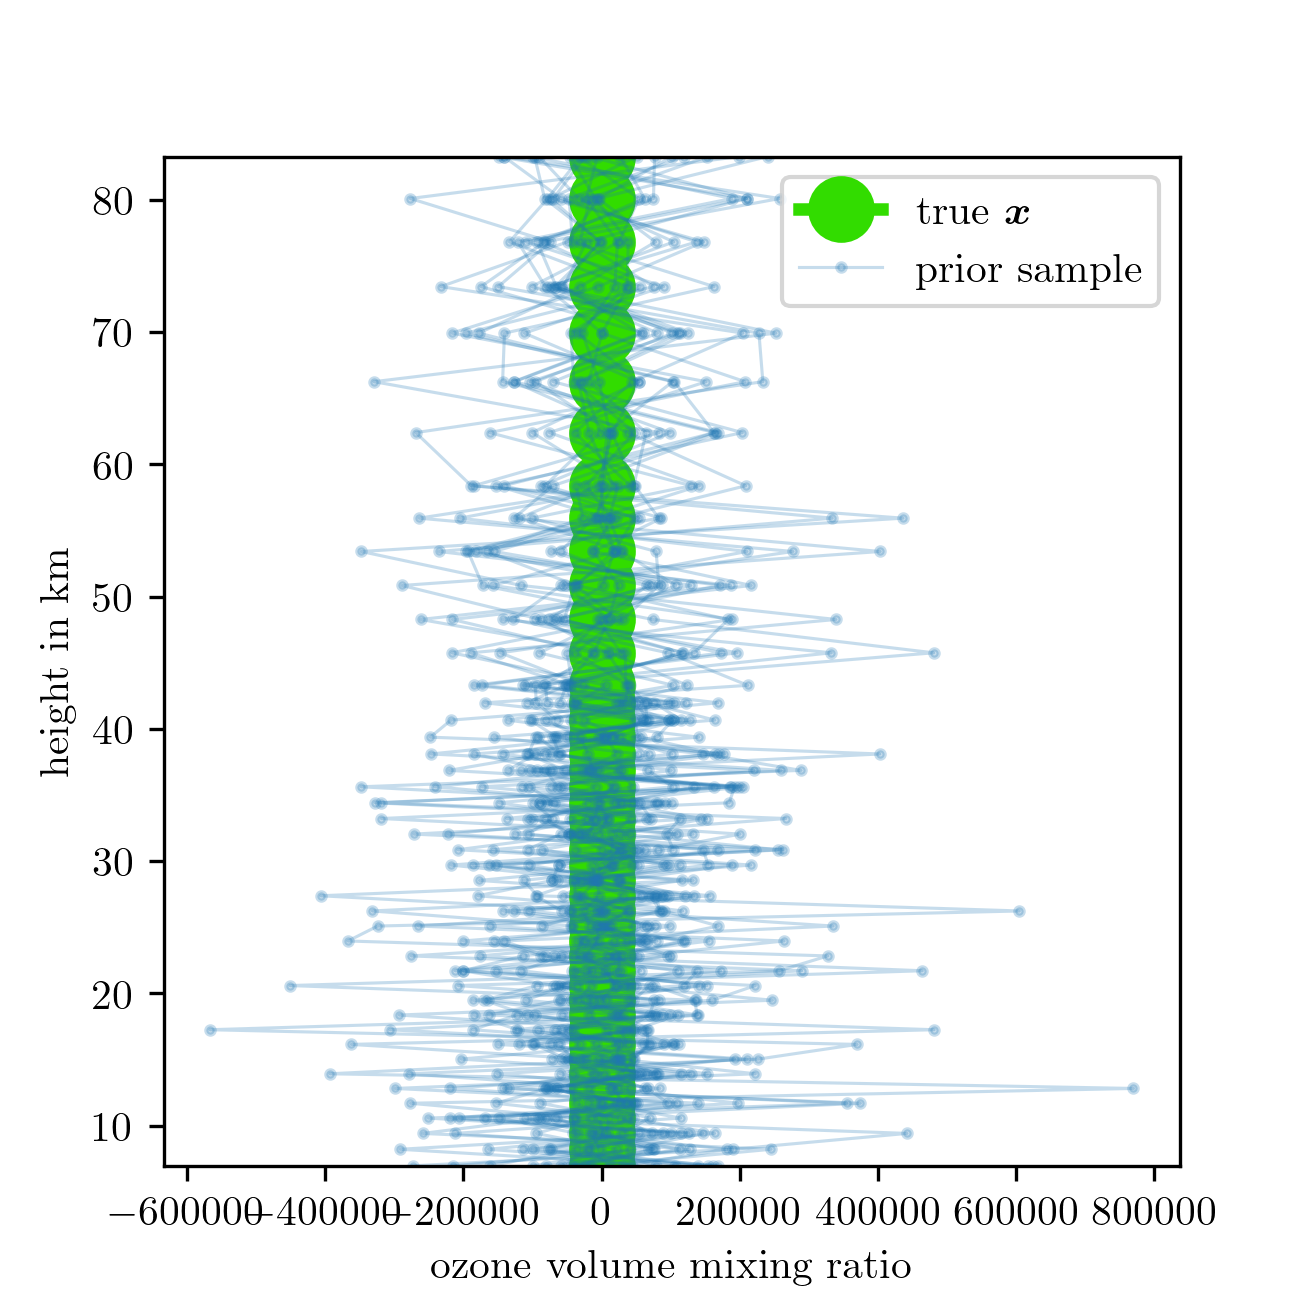
\includegraphics{OzonePrior.png}
	\caption[Samples from ozone prior distribution.]{We draw samples from ozone prior distribution $\bm{x} \sim \mathcal{N}(0,\delta \bm{L})$ after generating a sample from the hyper-prior distribution $\delta \sim \mathcal{T}(1,10^{-10})$. Note that since the variance of prior samples is very large compared to the ozone volume mixing ratios, the ozone profile appears to be constant, which is not the case, see e.g. Fig. \ref{fig:O3Samp}.}
	\label{fig:O3Prior}
\end{figure}


\subsection{Integrated Autocorrelation plots} 
\begin{figure}[ht!]
	\centering
	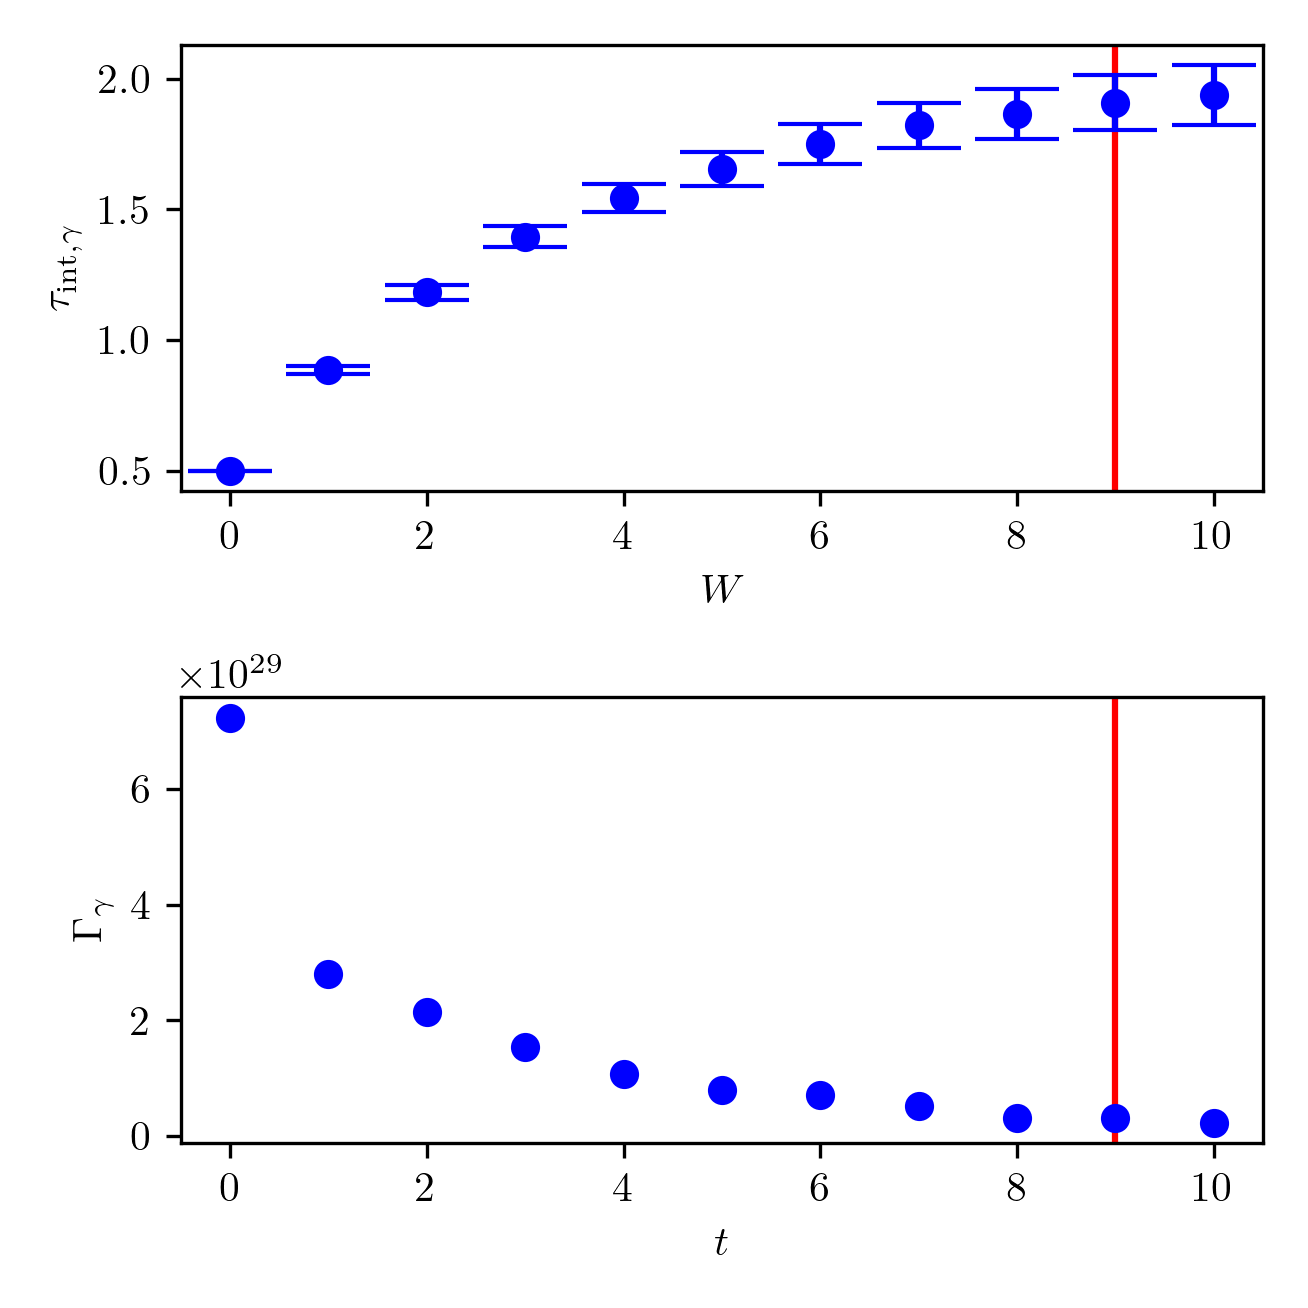
\includegraphics{UwerrTauIntFirstO3gam.png}
	\caption[IATC of $\gamma$ samples from $\pi(\gamma, \lambda| \bm{y})$, for linear model.]{Here the autocorrelation function $\Gamma_{\gamma}$ at different lags W is plotted as well as the IATC $\tau_{\text{int},\gamma}$ for the samples from $\pi(\gamma, \lambda| \bm{y})$ based on the linear forward model.}
	\label{fig:IATCGamLin}
\end{figure}
\begin{figure}[ht!]
	\centering
	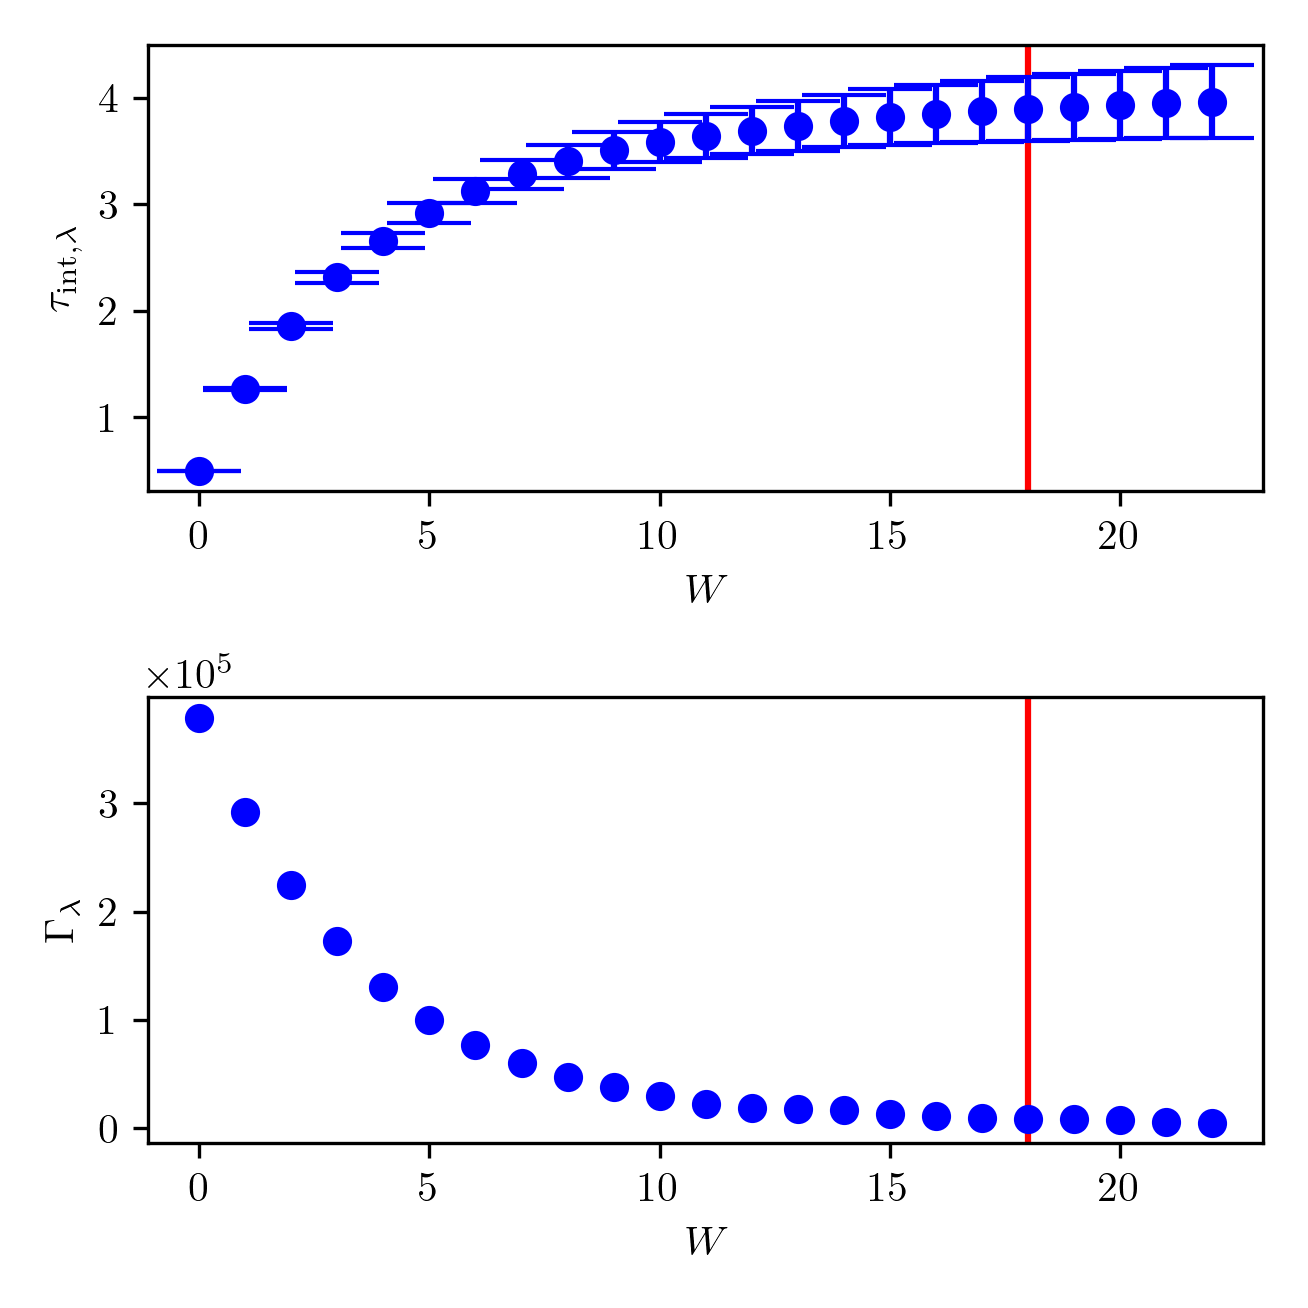
\includegraphics{UwerrTauIntSecO3lam.png}
	\caption[IACT and autocorrelation function for samples $\lambda \sim \pi{\cdot | \gamma, \bm{y}}$.]{IACT for samples $\lambda \sim \pi( \cdot | \gamma, \bm{y})$ based on the approximated forward model.}
	\label{fig:}
\end{figure}
\begin{figure}[ht!]
	\centering
	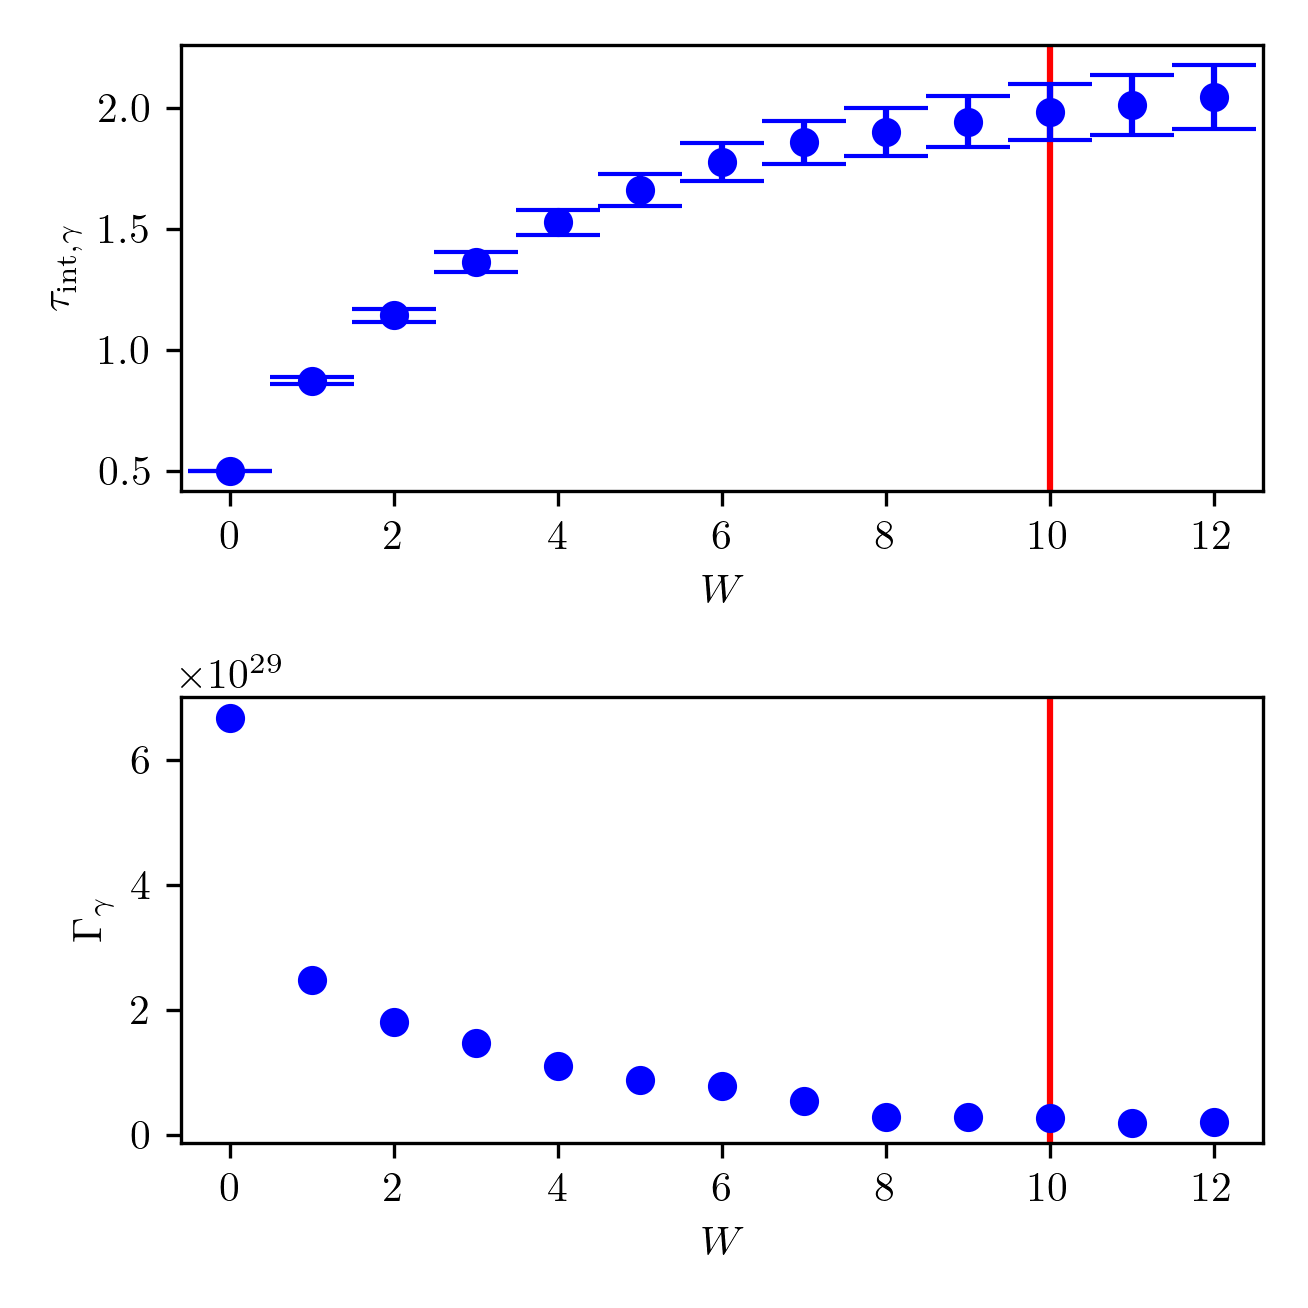
\includegraphics{UwerrTauIntSecO3gam.png}
	\caption[IACT and autocorrelation function for samples $\gamma \sim \pi( \cdot | \lambda, \bm{y})$]{IACT for samples $\gamma \sim \pi( \cdot | \lambda, \bm{y})$ based on the approximated forward model.}
	\label{fig:}
\end{figure}
\clearpage
\section{Pressure and Temperature}

\subsection{Priors}
\begin{figure}[ht!]
	\centering
	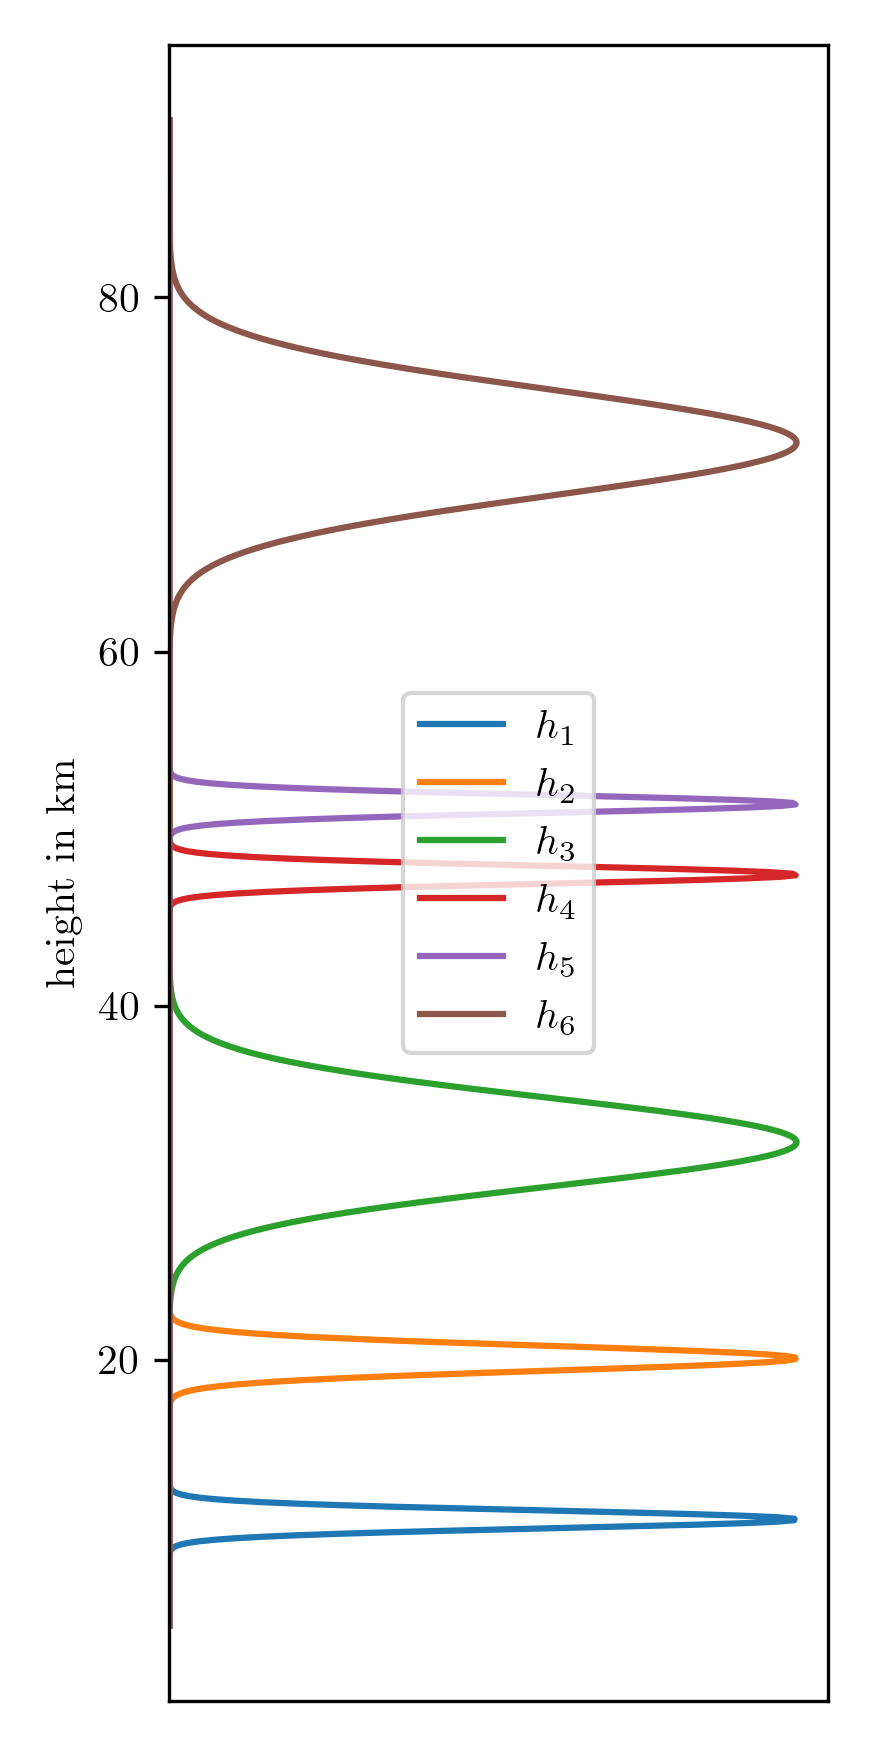
\includegraphics{HeightPriors.png}
	\caption[Prior distributions $\pi(\bm{h_T})$.]{Prior distributions $\pi(\bm{h_T})$, which we choose so that they do not overlap and not conflict with the temperature function \ref{eq:tempFunc}}
	\label{fig:HeightPriors}
\end{figure} 

\begin{figure}[ht!]
	\centering
	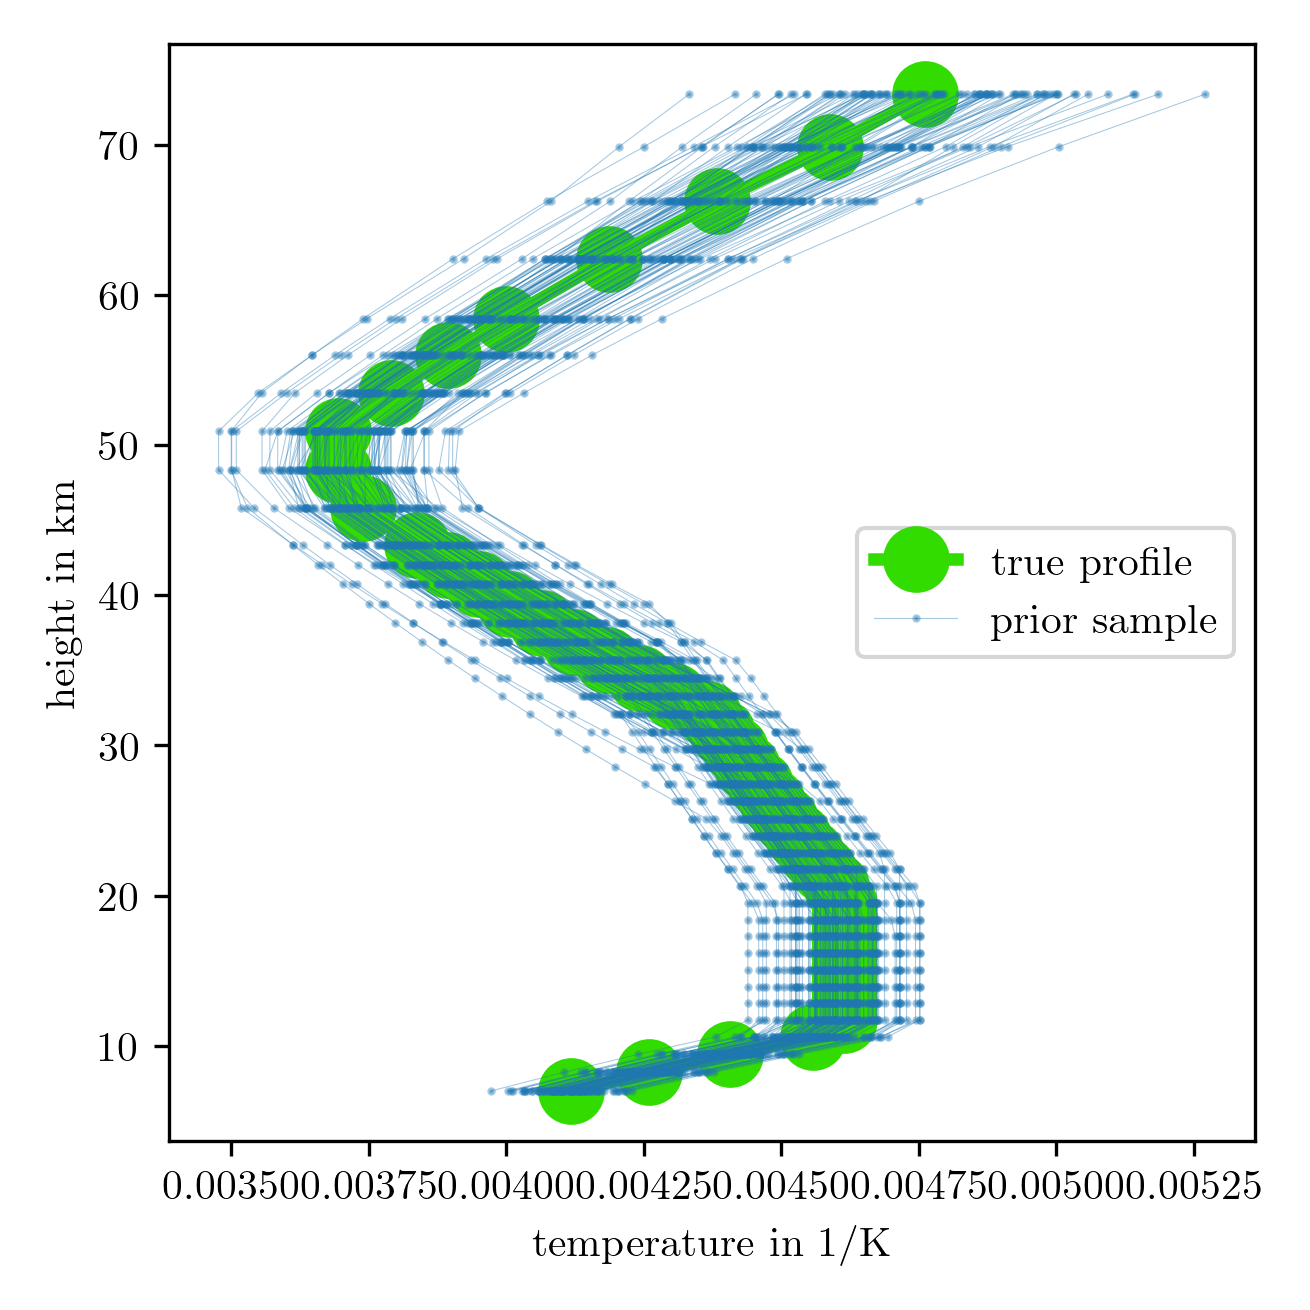
\includegraphics{PriorOverTempPost.png}
	\caption[Prior samples of $1/\bm{T}$]{Prior samples of the inverted temperature profile.}
	\label{fig:OverTempPrior}
\end{figure}
\subsection{T-walk Trace}
\begin{figure}[ht!]
	\centering
	\includegraphics{TraceTwalk.png}
	\caption[T-walk trace]{Output trace of the t-walk on the posterior distribution $\pi(p_0,b,\bm{h_T},\bm{a}| \gamma,\bm{y})$.}
	\label{fig:TraceTwalk}
\end{figure}

\subsection{Integrated Autocorrelation Plots} 
\begin{figure}[ht!]
	\centering
	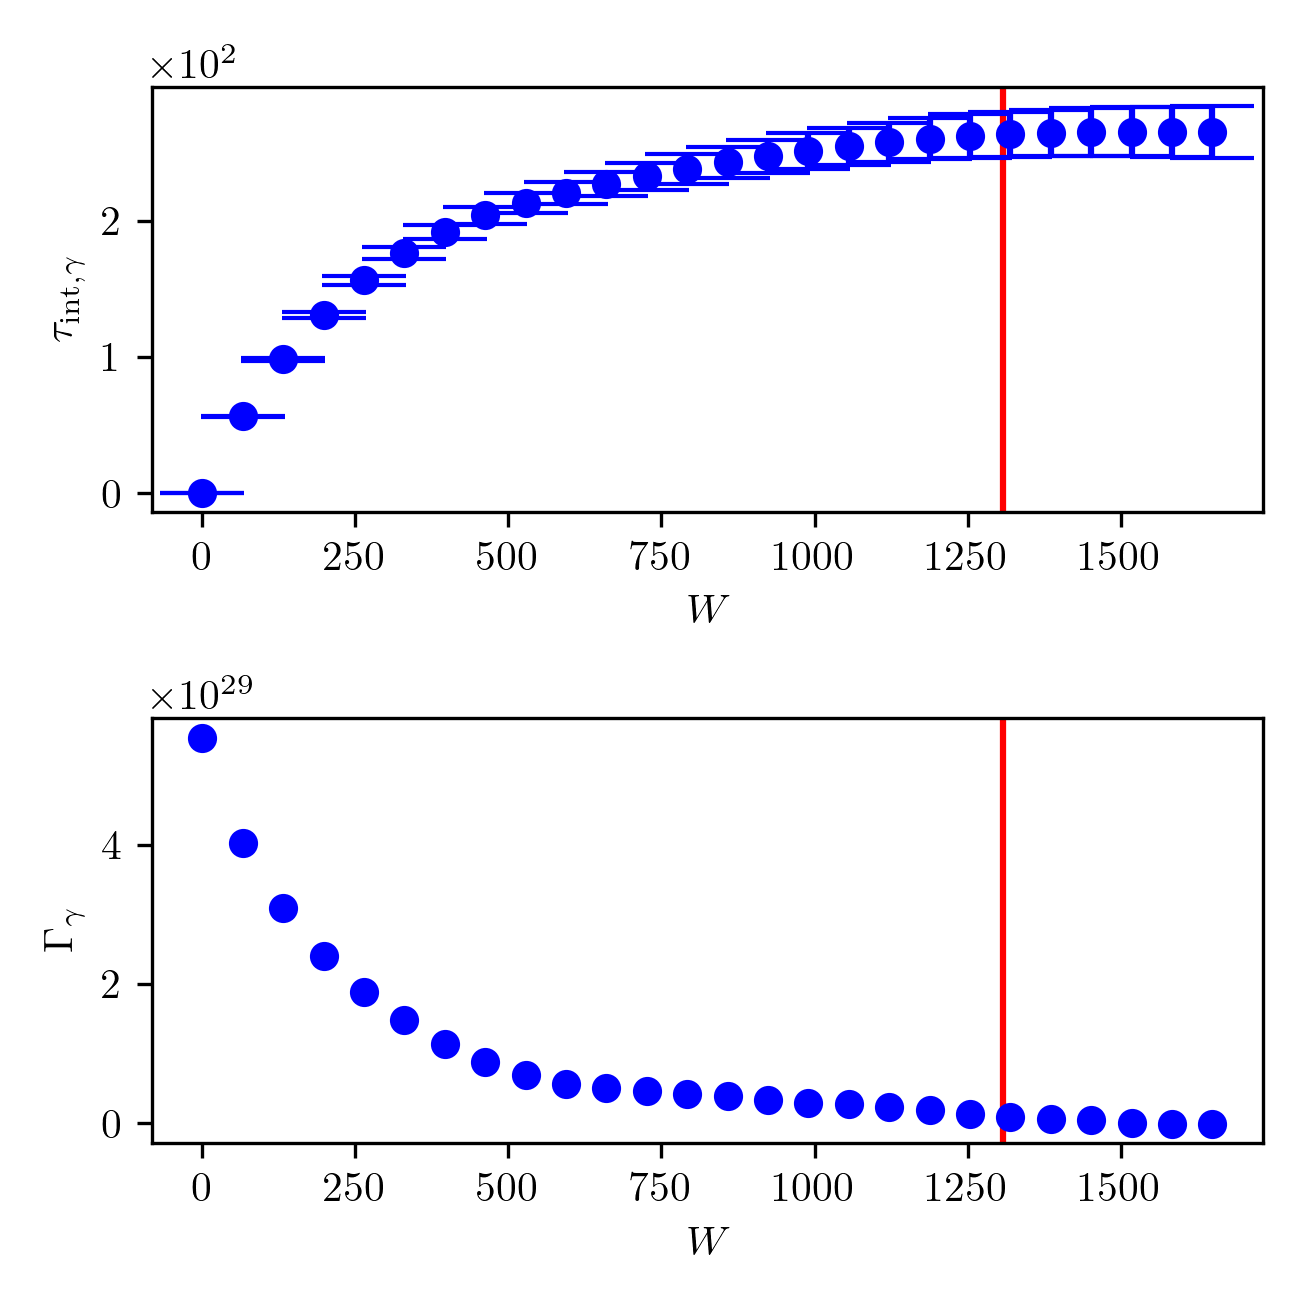
\includegraphics{UwerrTauIntTWalk0.png}
	\caption[IACT and autocorrelation function for $h_{T,1}$ samples.]{IACT and autocorrelation function for samples $h_1 \sim \pi( \cdot |h_{T,2},h_{T,3},h_{T,4},h_{T,5},h_{T,6},a_0,a_1,a_2,a_3,a_4,a_5,a_6,T_0,b,p_0, \bm{y})$}
	\label{fig:}
\end{figure}
\begin{figure}[ht!]
	\centering
	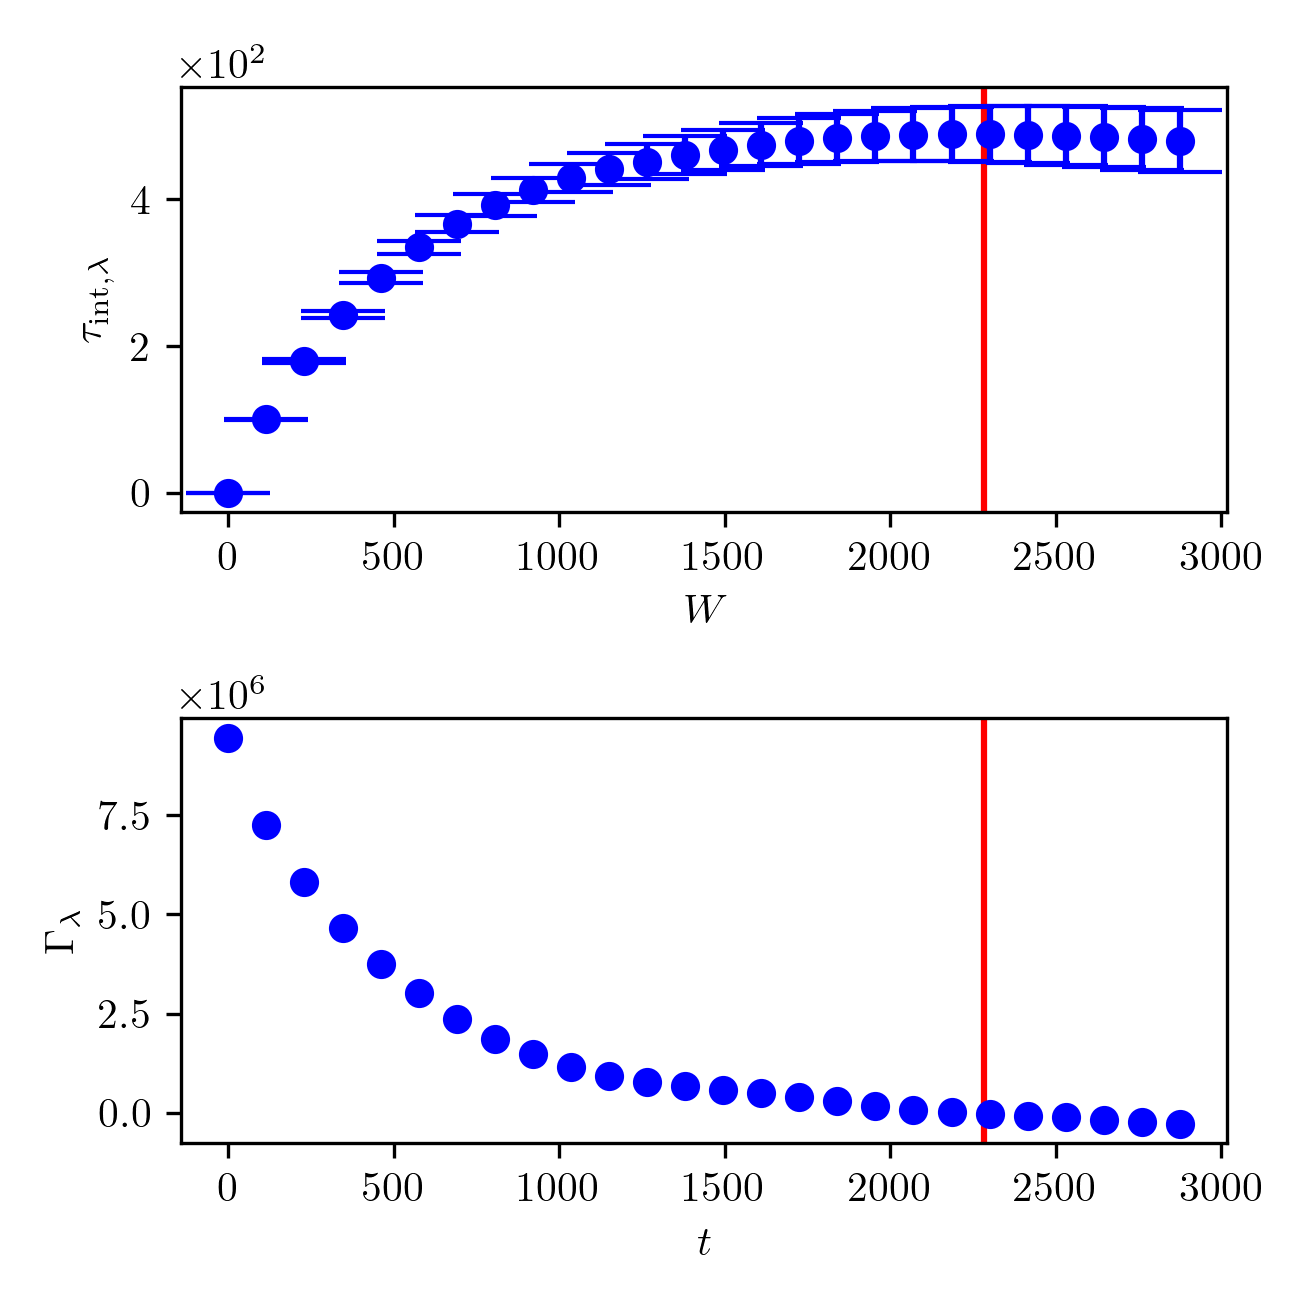
\includegraphics{UwerrTauIntTWalk1.png}
	\caption[IACT and autocorrelation function for $h_2$ samples.]{IACT and autocorrelation function for samples $h_2 \sim \pi( \cdot | h_1,h_3,h_4,h_5,h_6,a_0,a_1,a_2,a_3,a_4,a_5,a_6,T_0,b,p_0, \bm{y})$}
	\label{fig:}
\end{figure}


\begin{figure}[ht!]
	\centering
	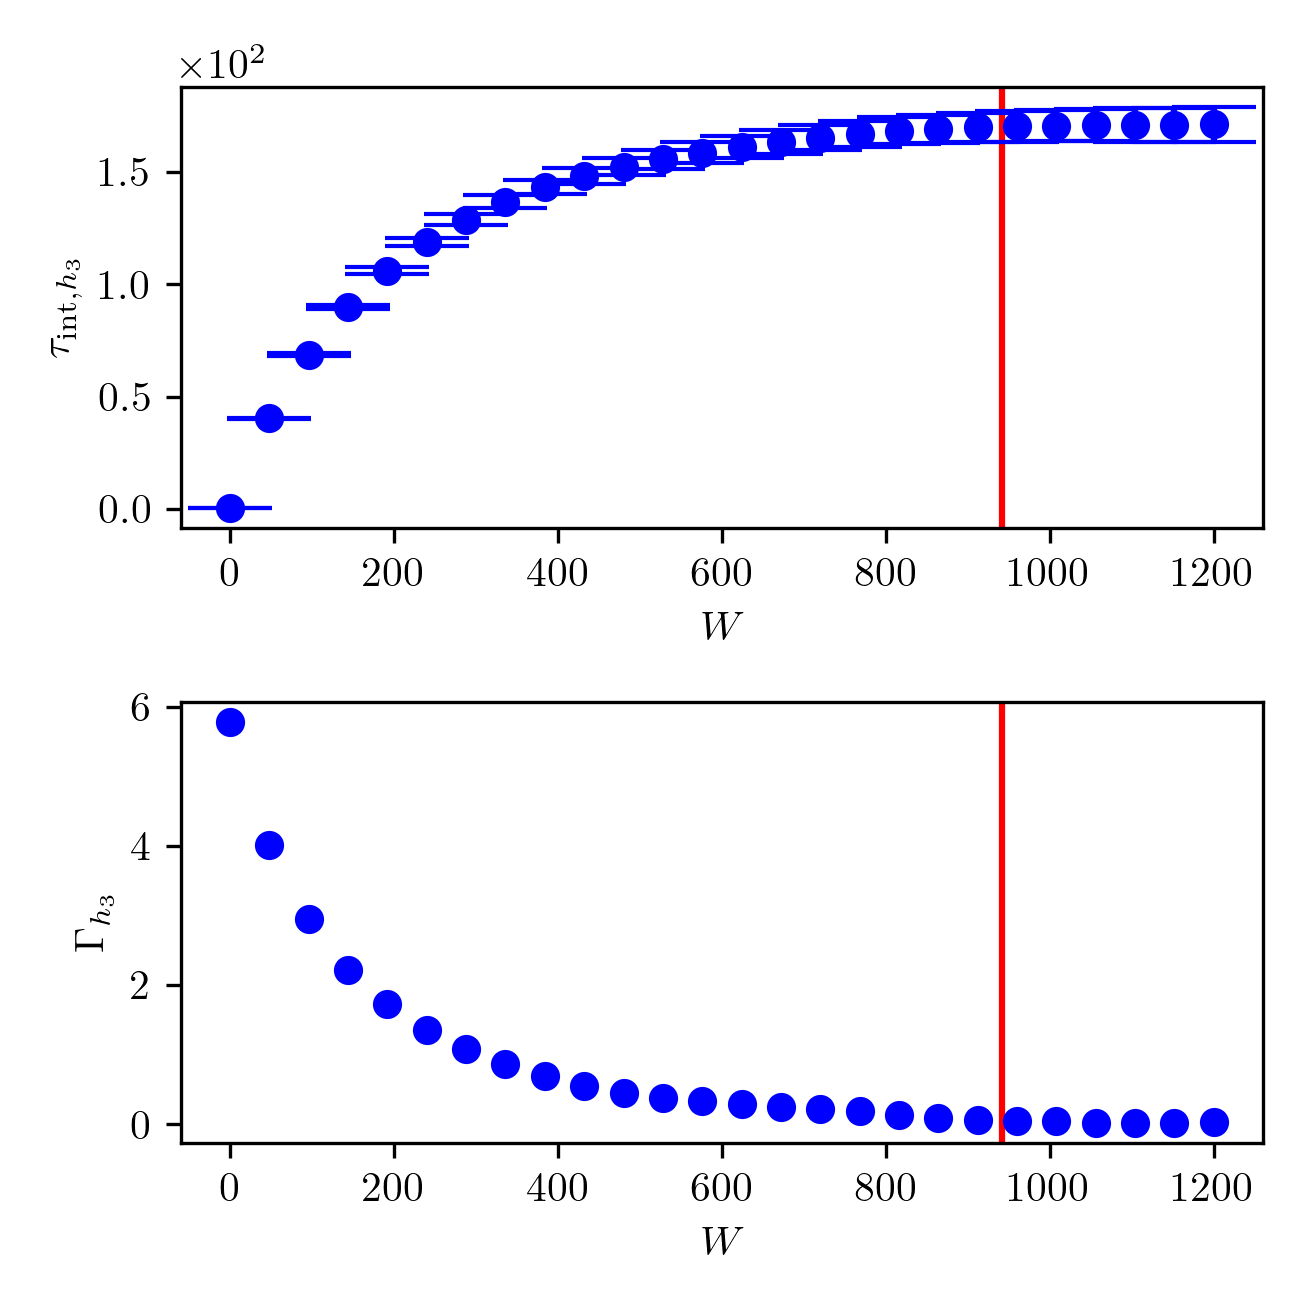
\includegraphics{UwerrTauIntTWalk2.png}
	\caption[IACT and autocorrelation function for $h_3$ samples.]{IACT and autocorrelation function for samples $h_3 \sim \pi( \cdot | h_1,h_2,h_4,h_5,h_6,a_0,a_1,a_2,a_3,a_4,a_5,a_6,T_0,b,p_0, \bm{y})$}
	\label{fig:}
\end{figure}


\begin{figure}[ht!]
	\centering
	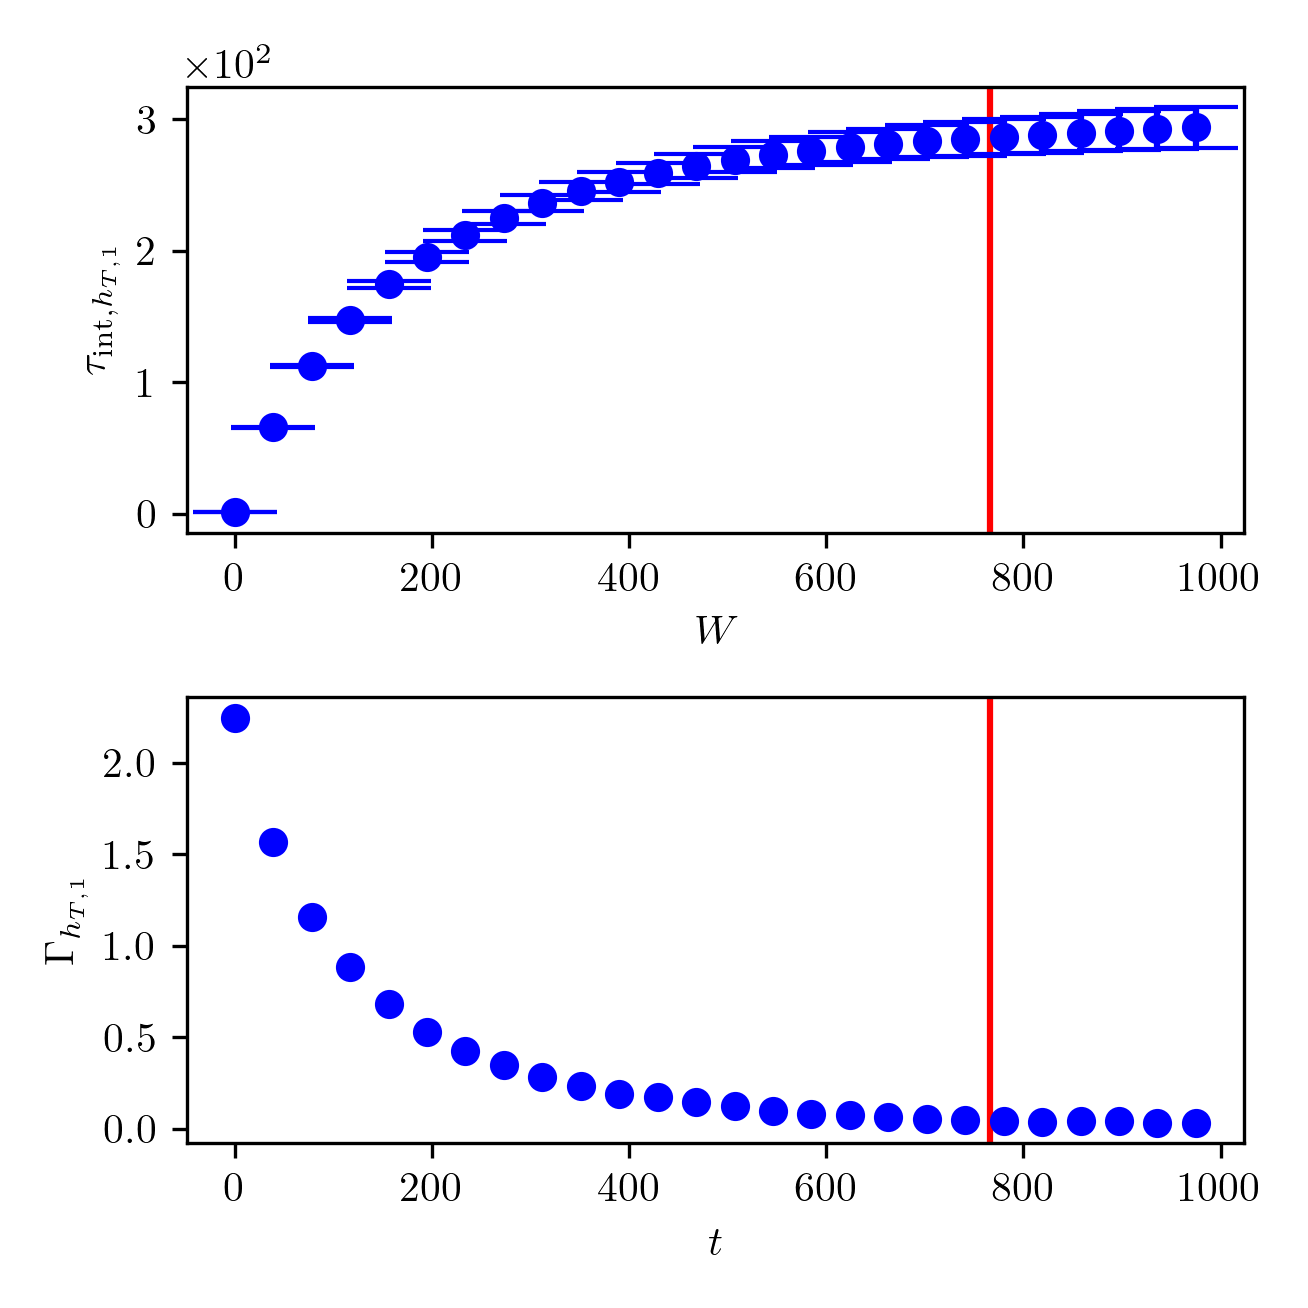
\includegraphics{UwerrTauIntTWalk3.png}
	\caption[IACT and autocorrelation function for $h_4$ samples.]{IACT and autocorrelation function for samples $h_4 \sim \pi( \cdot | h_1,h_2,h_3,h_5,h_6,a_0,a_1,a_2,a_3,a_4,a_5,a_6,T_0,b,p_0, \bm{y})$}
	\label{fig:}
\end{figure}


\begin{figure}[ht!]
	\centering
	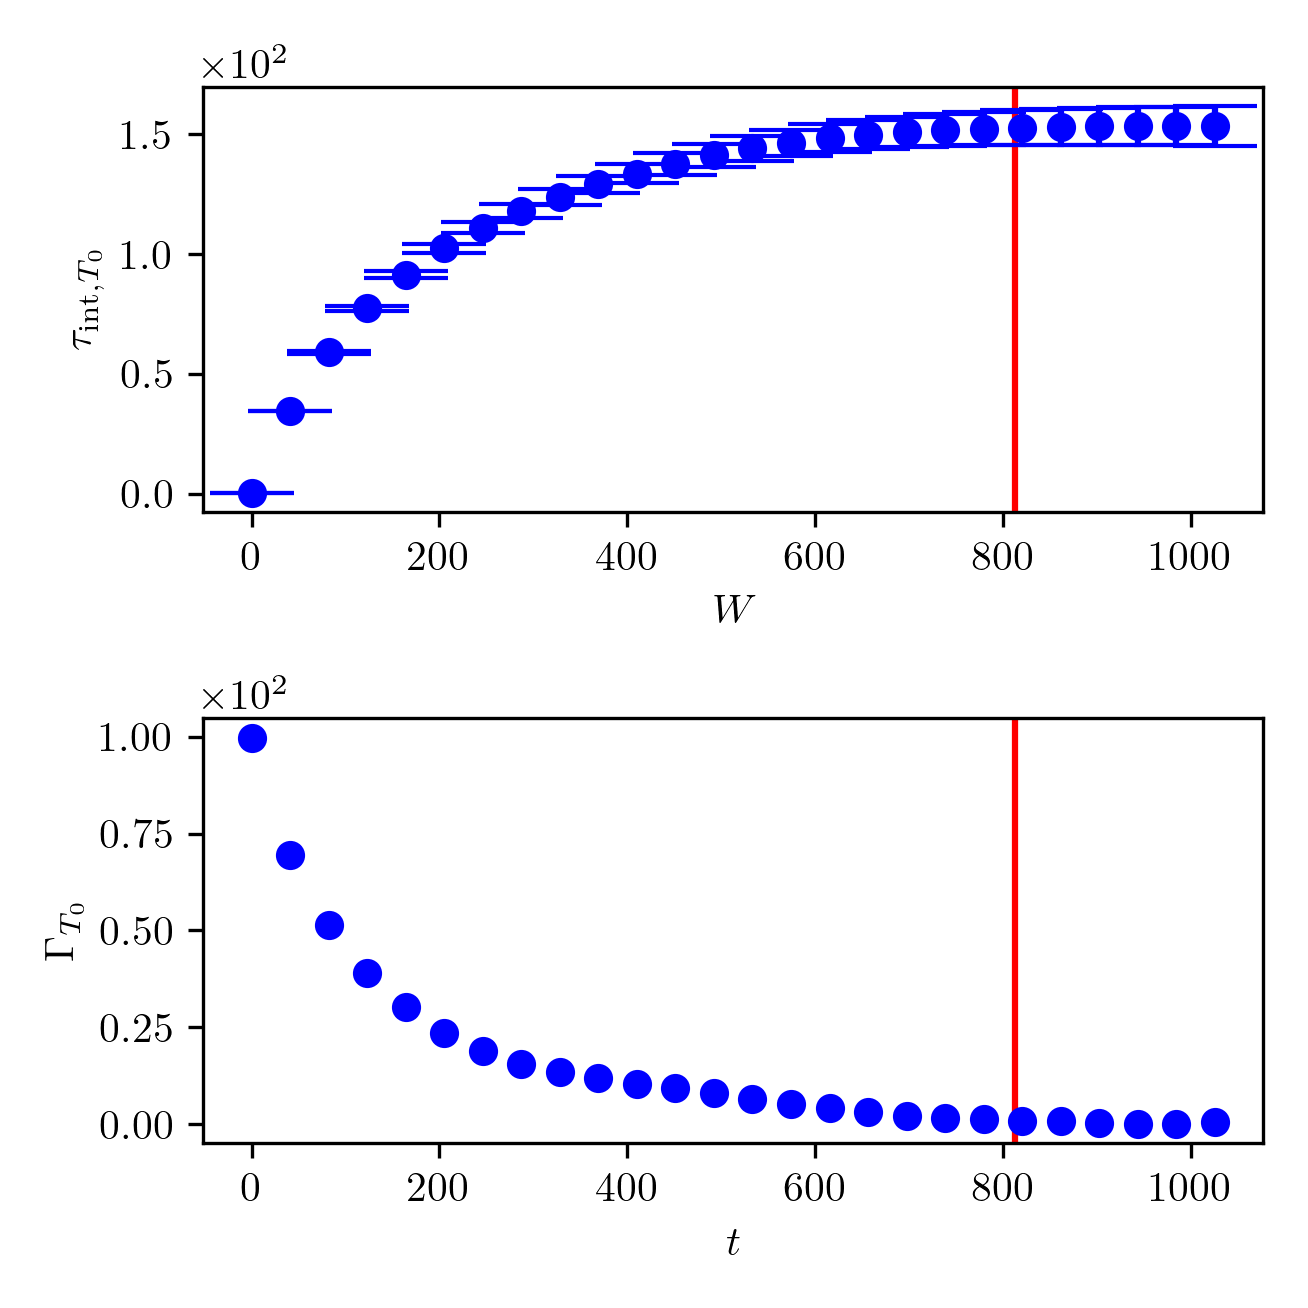
\includegraphics{UwerrTauIntTWalk4.png}
	\caption[IACT and autocorrelation function for $h_5$ samples.]{IACT and autocorrelation function for samples $h_5 \sim \pi( \cdot | h_1, h_2,h_3,h_4,h_6,a_0,a_1,a_2,a_3,a_4,a_5,a_6,T_0,b,p_0,  \bm{y})$}
	\label{fig:}
\end{figure}


\begin{figure}[ht!]
	\centering
	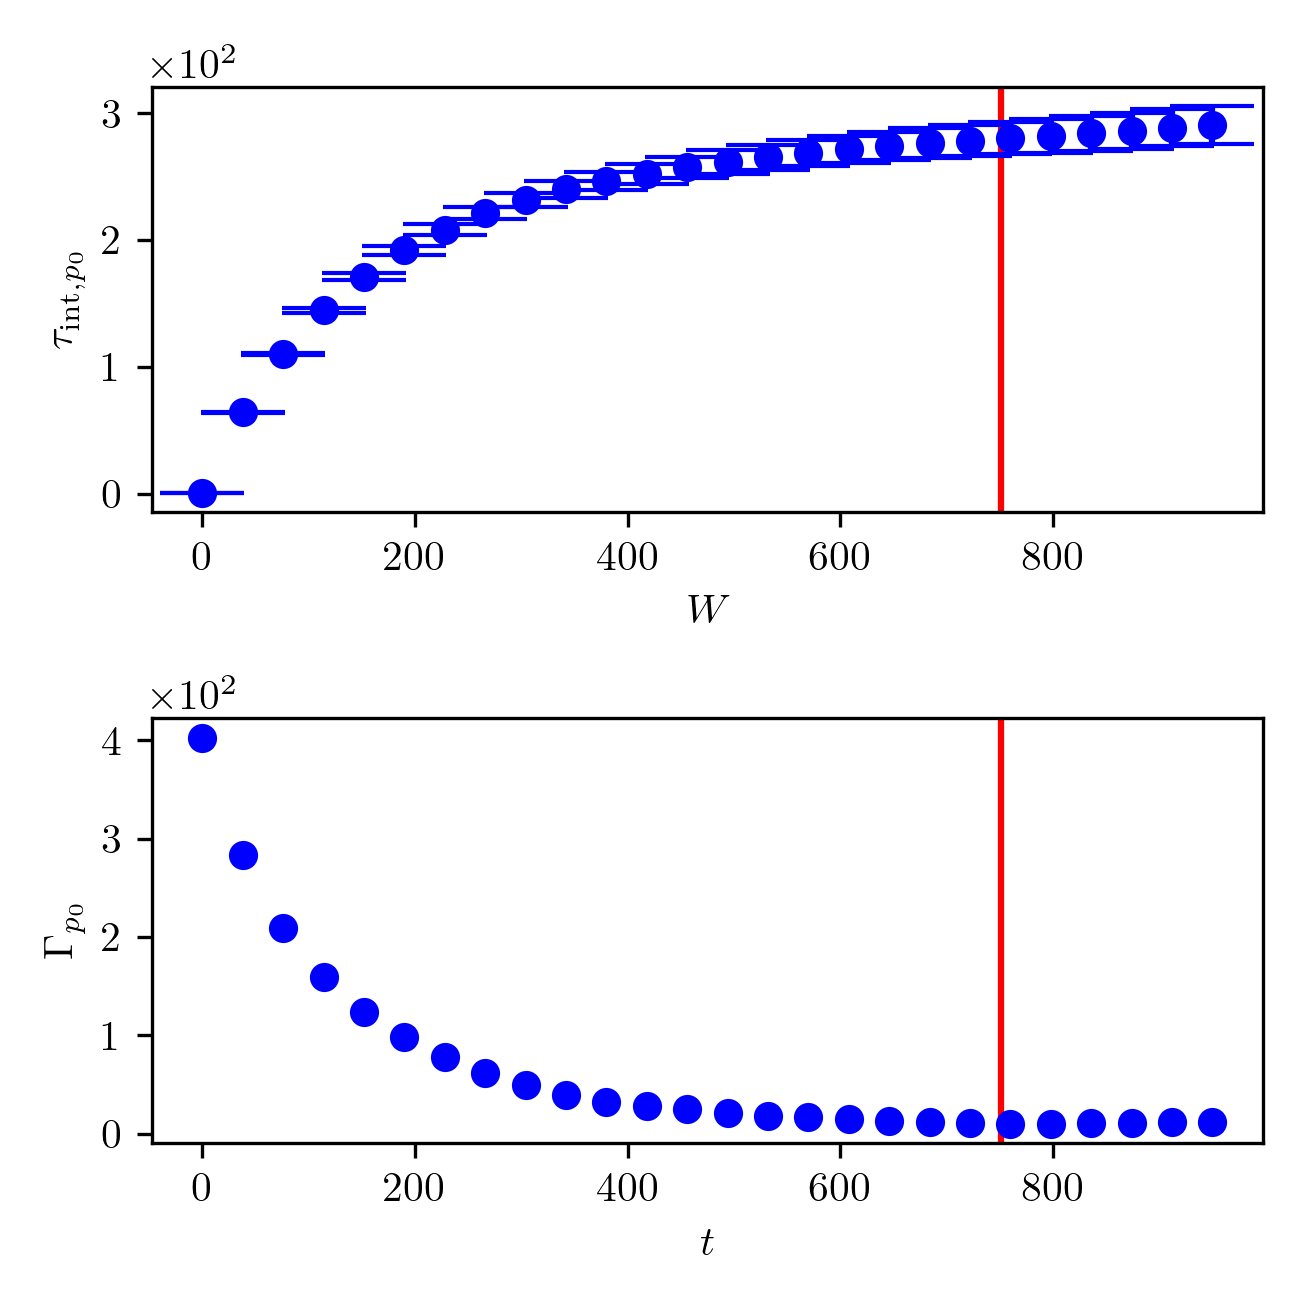
\includegraphics{UwerrTauIntTWalk5.png}
	\caption[IACT and autocorrelation function for $h_6$ samples.]{IACT and autocorrelation function for samples $h_6 \sim \pi( \cdot | h_1, h_2,h_3,h_4,h_5,a_0,a_1,a_2,a_3,a_4,a_5,a_6,T_0,b,p_0,  \bm{y})$}
	\label{fig:}
\end{figure}


\begin{figure}[ht!]
	\centering
	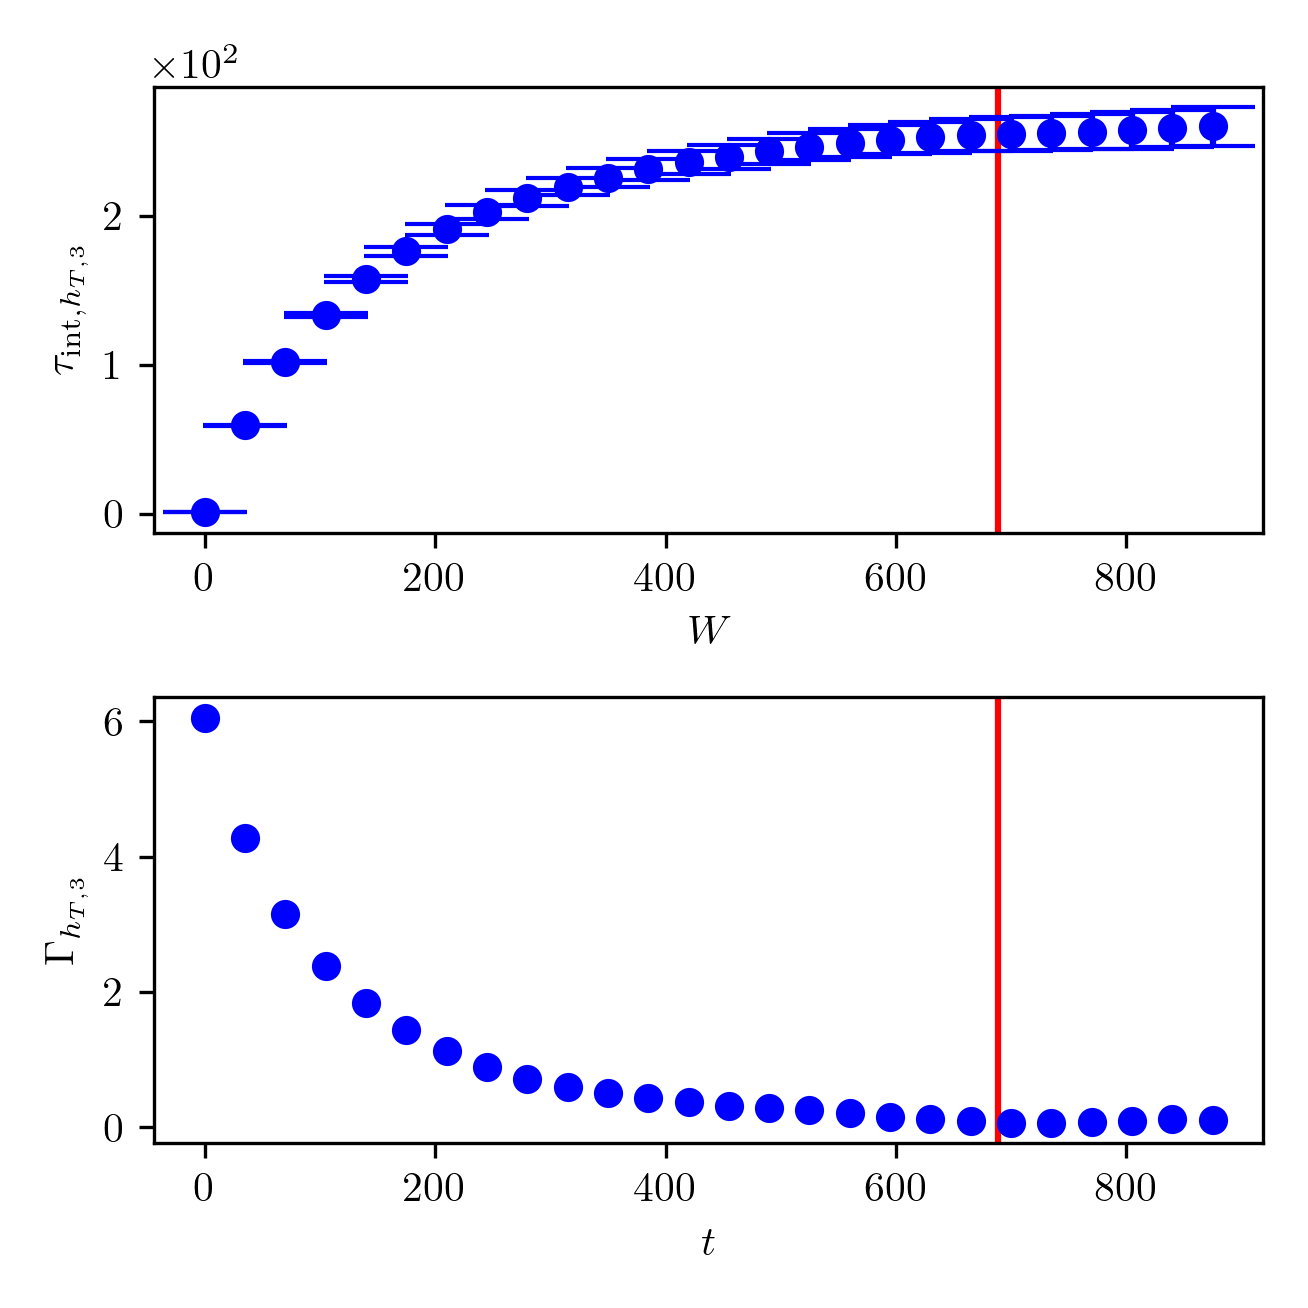
\includegraphics{UwerrTauIntTWalk6.png}
	\caption[IACT and autocorrelation function for $a_0$ samples.]{IACT and autocorrelation function for samples $a_0 \sim \pi( \cdot | h_1, h_2,h_3,h_4,h_5,h_6,a_1,a_2,a_3,a_4,a_5,a_6,T_0,b,p_0,  \bm{y})$}
	\label{fig:}
\end{figure}

\begin{figure}[ht!]
	\centering
	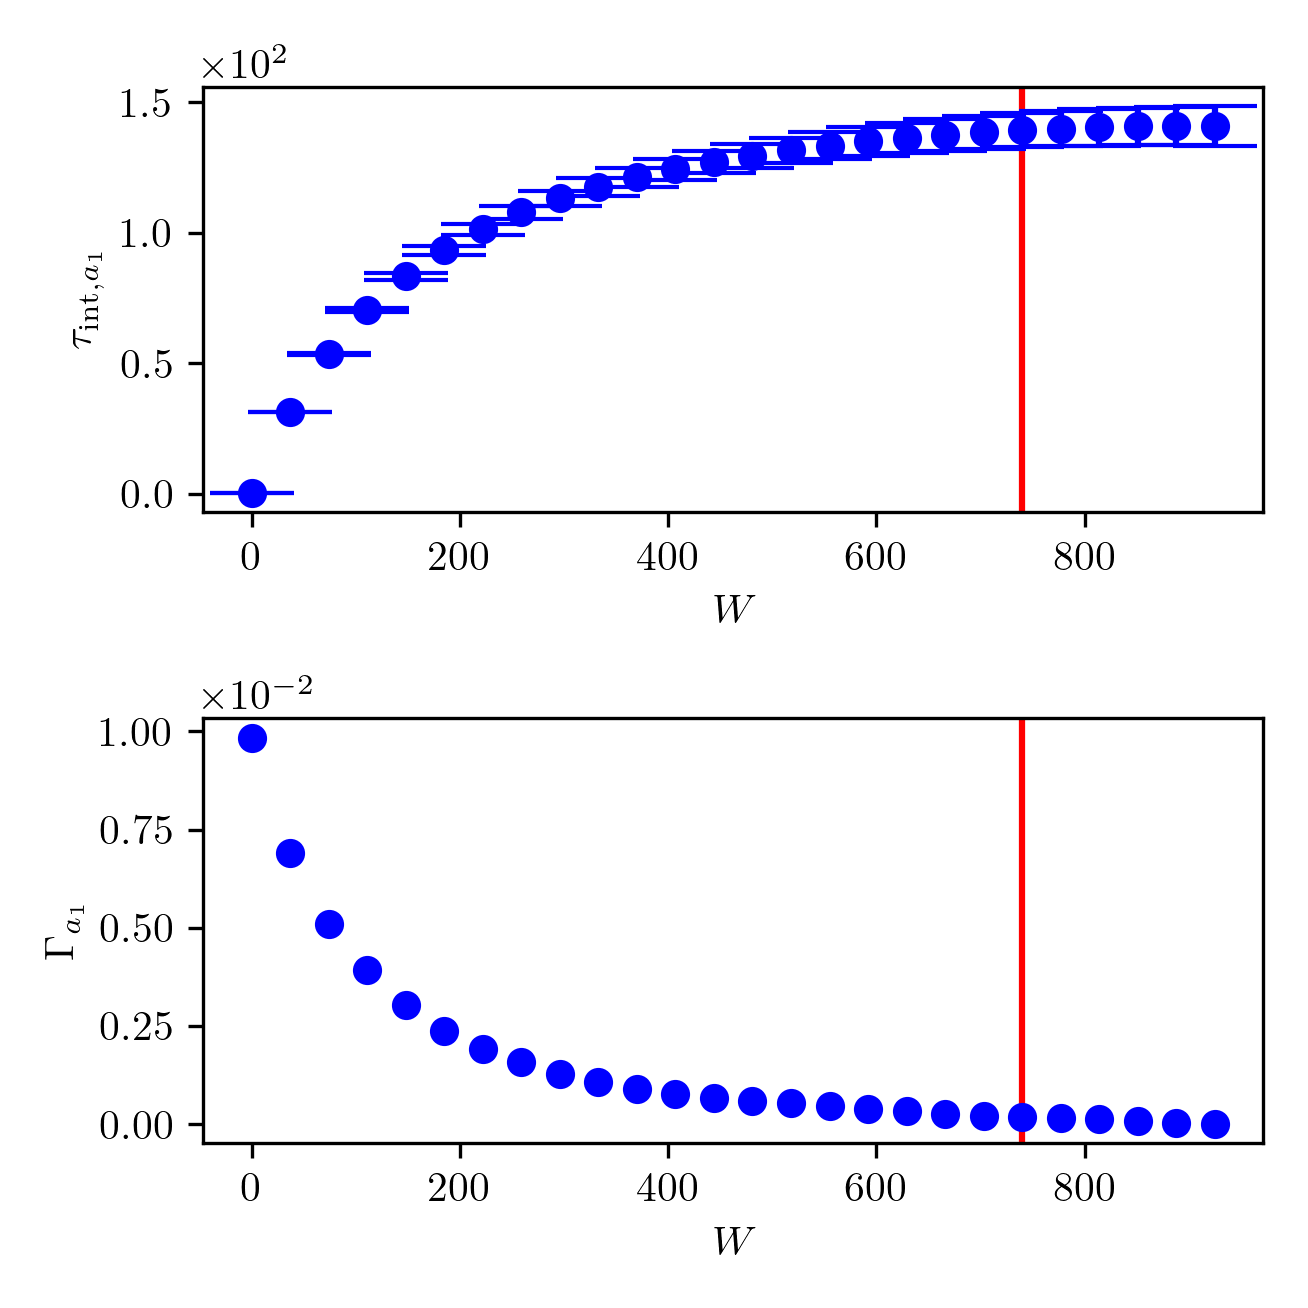
\includegraphics{UwerrTauIntTWalk7.png}
	\caption[IACT and autocorrelation function for $a_1$ samples.]{IACT and autocorrelation function for samples $a_1 \sim \pi( \cdot | h_1, h_2,h_3,h_4,h_5,h_6,a_0,a_2,a_3,a_4,a_5,a_6,T_0,b,p_0,  \bm{y})$}
	\label{fig:}
\end{figure}


\begin{figure}[ht!]
	\centering
	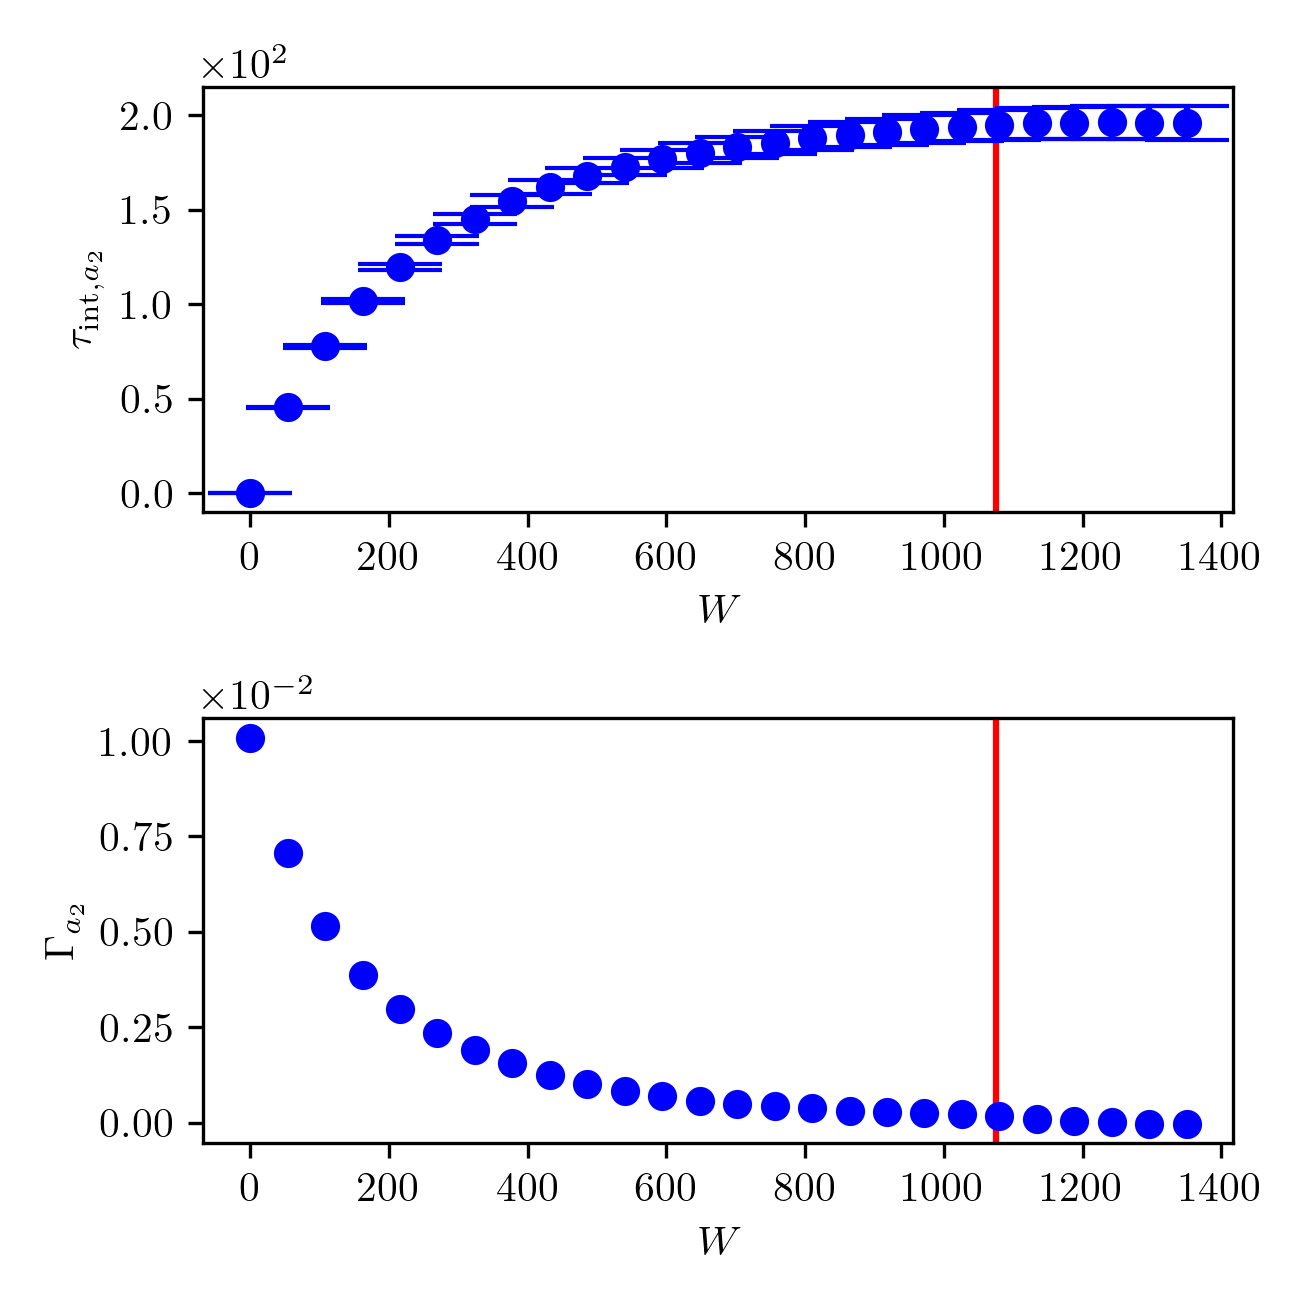
\includegraphics{UwerrTauIntTWalk8.png}
	\caption[IACT and autocorrelation function for $a_2$ samples.]{IACT and autocorrelation function for samples $a_2 \sim \pi( \cdot | h_1, h_2,h_3,h_4,h_5,h_6,a_0,a_1,a_3,a_4,a_5,a_6,T_0,b,p_0,  \bm{y})$}
	\label{fig:}
\end{figure}


\begin{figure}[ht!]
	\centering
	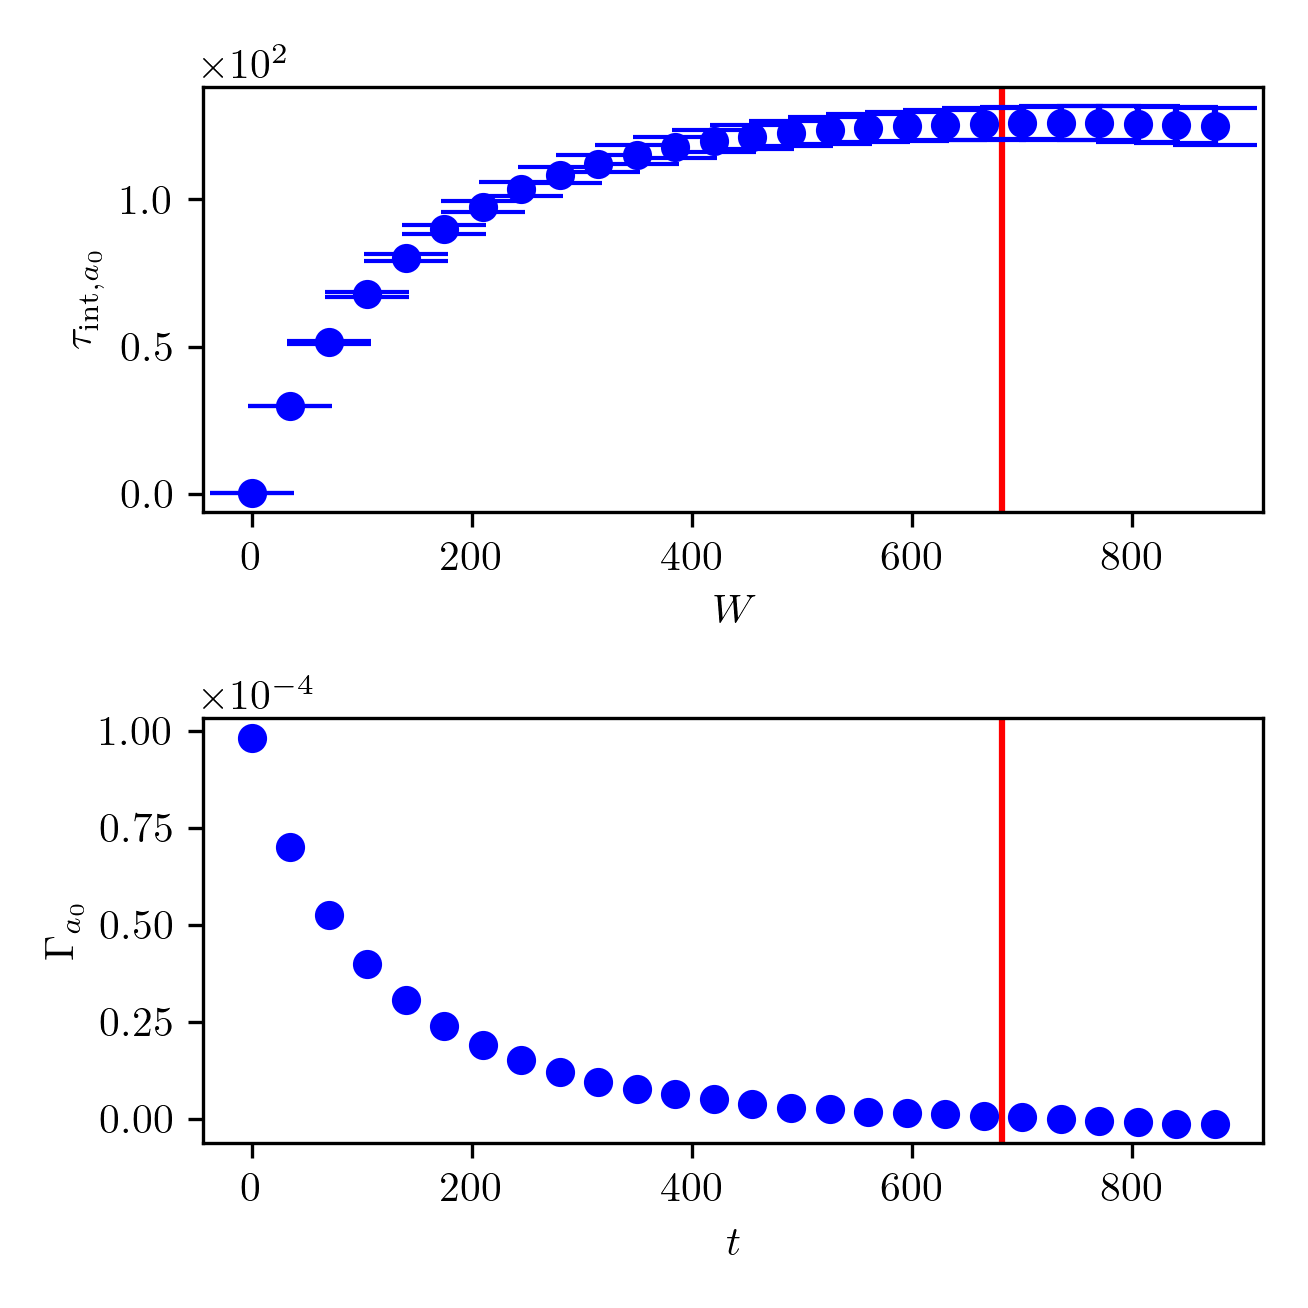
\includegraphics{UwerrTauIntTWalk9.png}
	\caption[IACT and autocorrelation function for $a_3$ samples.]{IACT and autocorrelation function for samples $a_3 \sim \pi( \cdot | h_1, h_2,h_3,h_4,h_5,h_6,a_0,a_1,a_2,a_4,a_5,a_6,T_0,b,p_0,  \bm{y})$}
	\label{fig:}
\end{figure}

\begin{figure}[ht!]
	\centering
	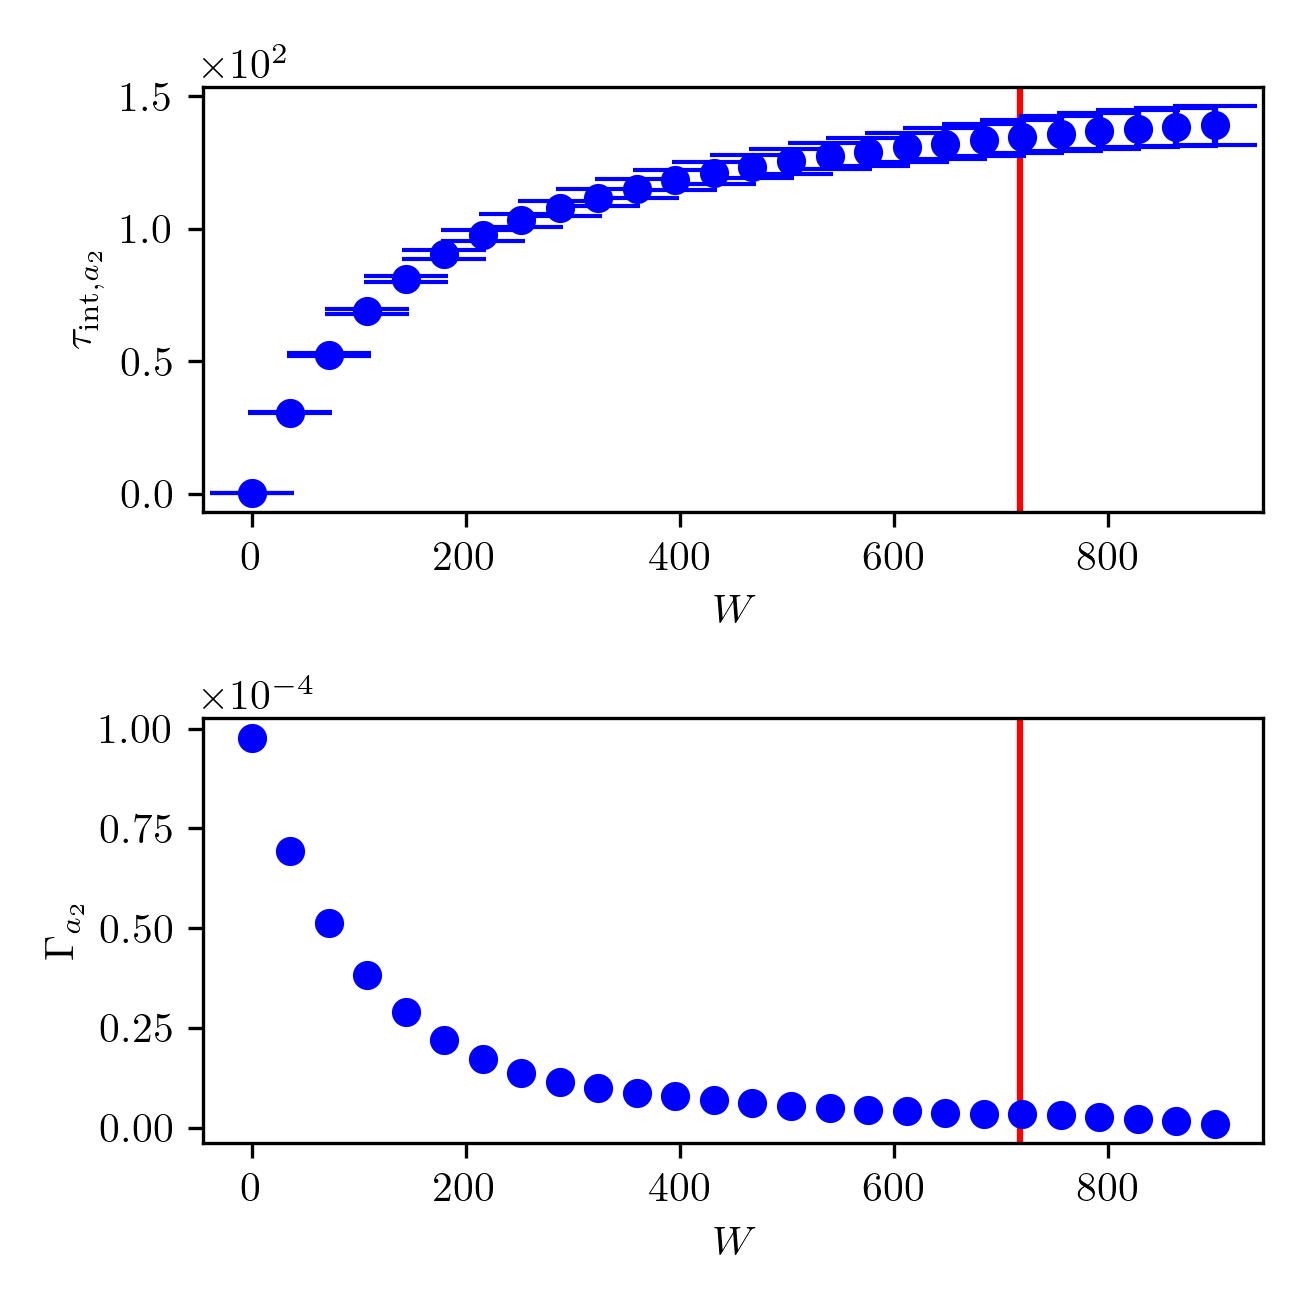
\includegraphics{UwerrTauIntTWalk10.png}
	\caption[IACT and autocorrelation function for $a_4 $ samples.]{IACT and autocorrelation function for samples $a_4 \sim \pi( \cdot | h_1, h_2,h_3,h_4,h_5,h_6,a_0,a_1,a_2,a_4,a_5,a_6,T_0,b,p_0,  \bm{y})$}
	\label{fig:}
\end{figure}


\begin{figure}[ht!]
	\centering
	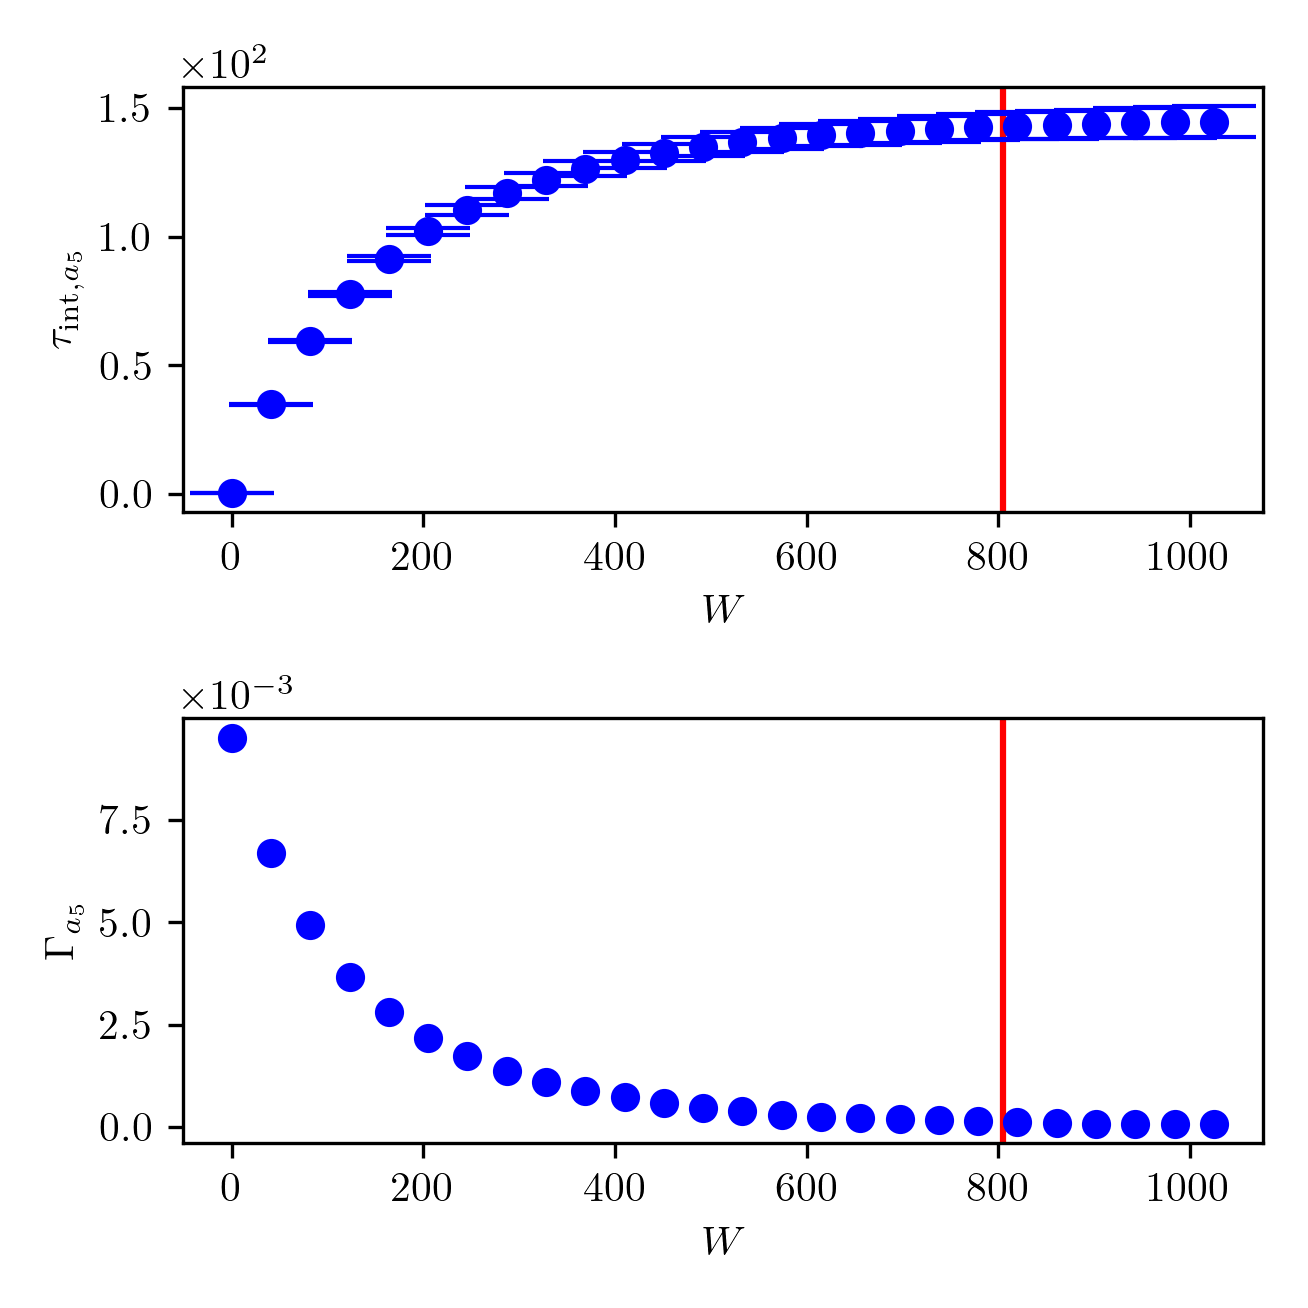
\includegraphics{UwerrTauIntTWalk11.png}
	\caption[IACT and autocorrelation function for $a_5$ samples.]{IACT and autocorrelation function for samples $a_5 \sim \pi( \cdot | h_1, h_2,h_3,h_4,h_5,h_6,a_0,a_1,a_2,a_3,a_4,a_5,T_0,b,p_0,  \bm{y})$}
	\label{fig:}
\end{figure}
\begin{figure}[ht!]
	\centering
	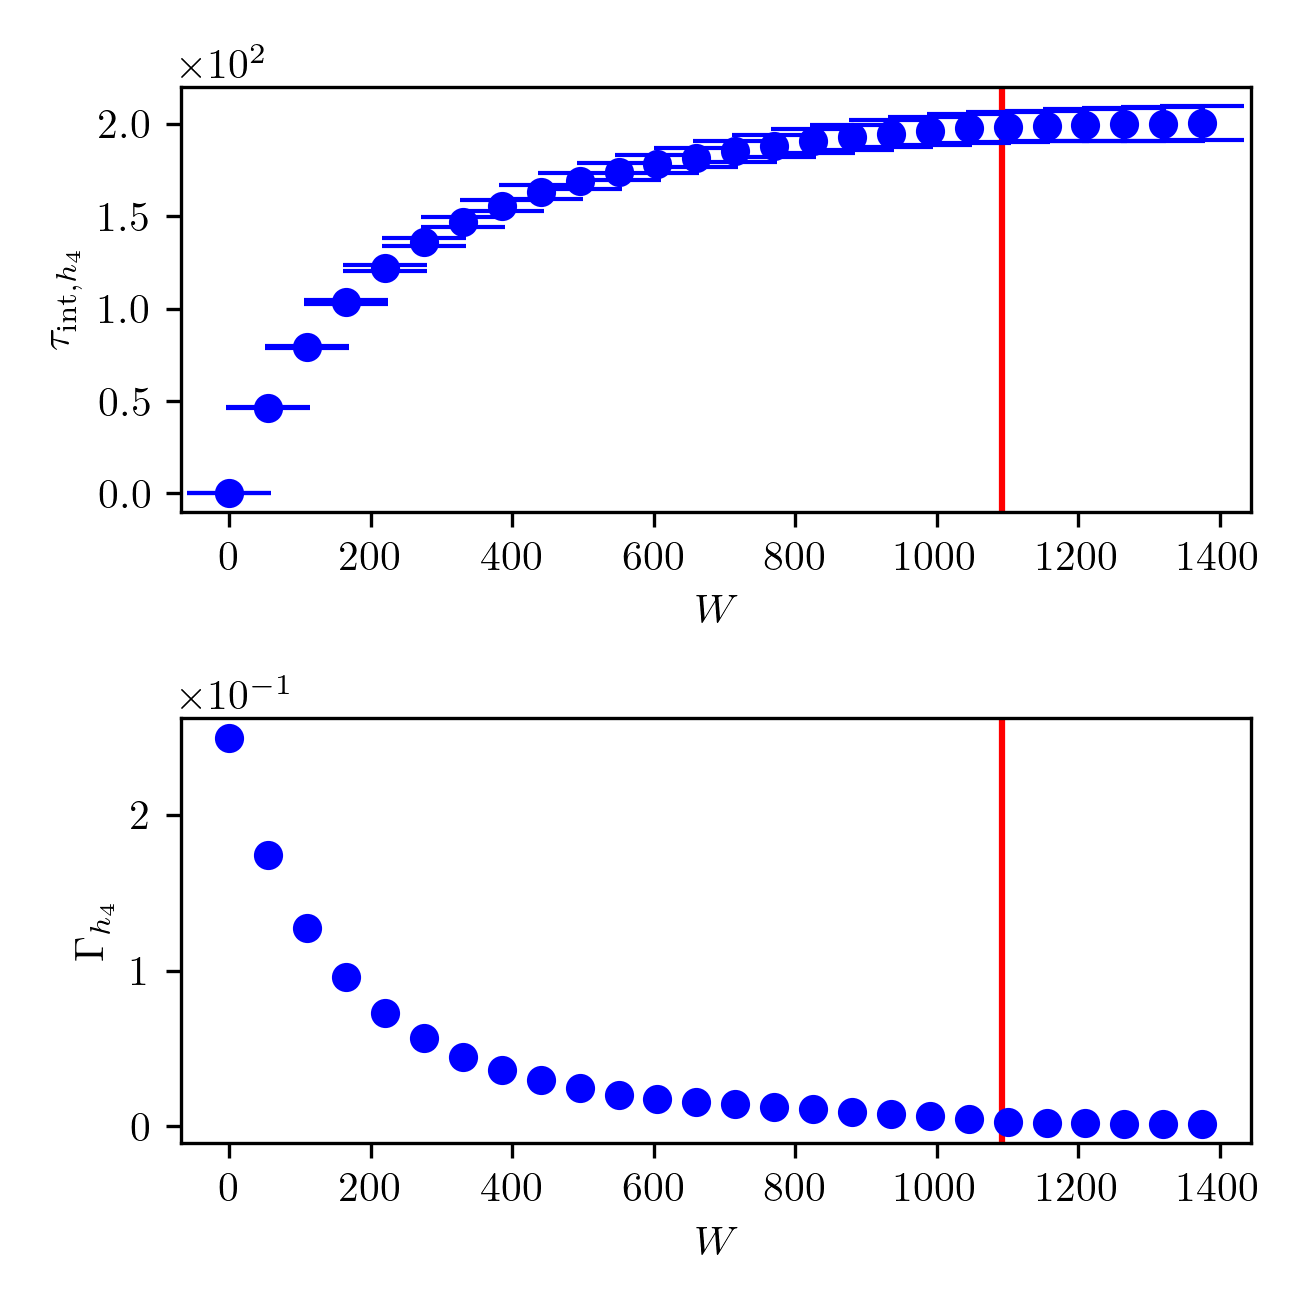
\includegraphics{UwerrTauIntTWalk12.png}
	\caption[IACT and autocorrelation function for $a_6$ samples.]{IACT and autocorrelation function for samples $a_6 \sim \pi( \cdot | h_1, h_2,h_3,h_4,h_5,h_6,a_0,a_1,a_2,a_3,a_4,a_5,T_0,b,p_0,  \bm{y})$}
	\label{fig:}
\end{figure}
\begin{figure}[ht!]
	\centering
	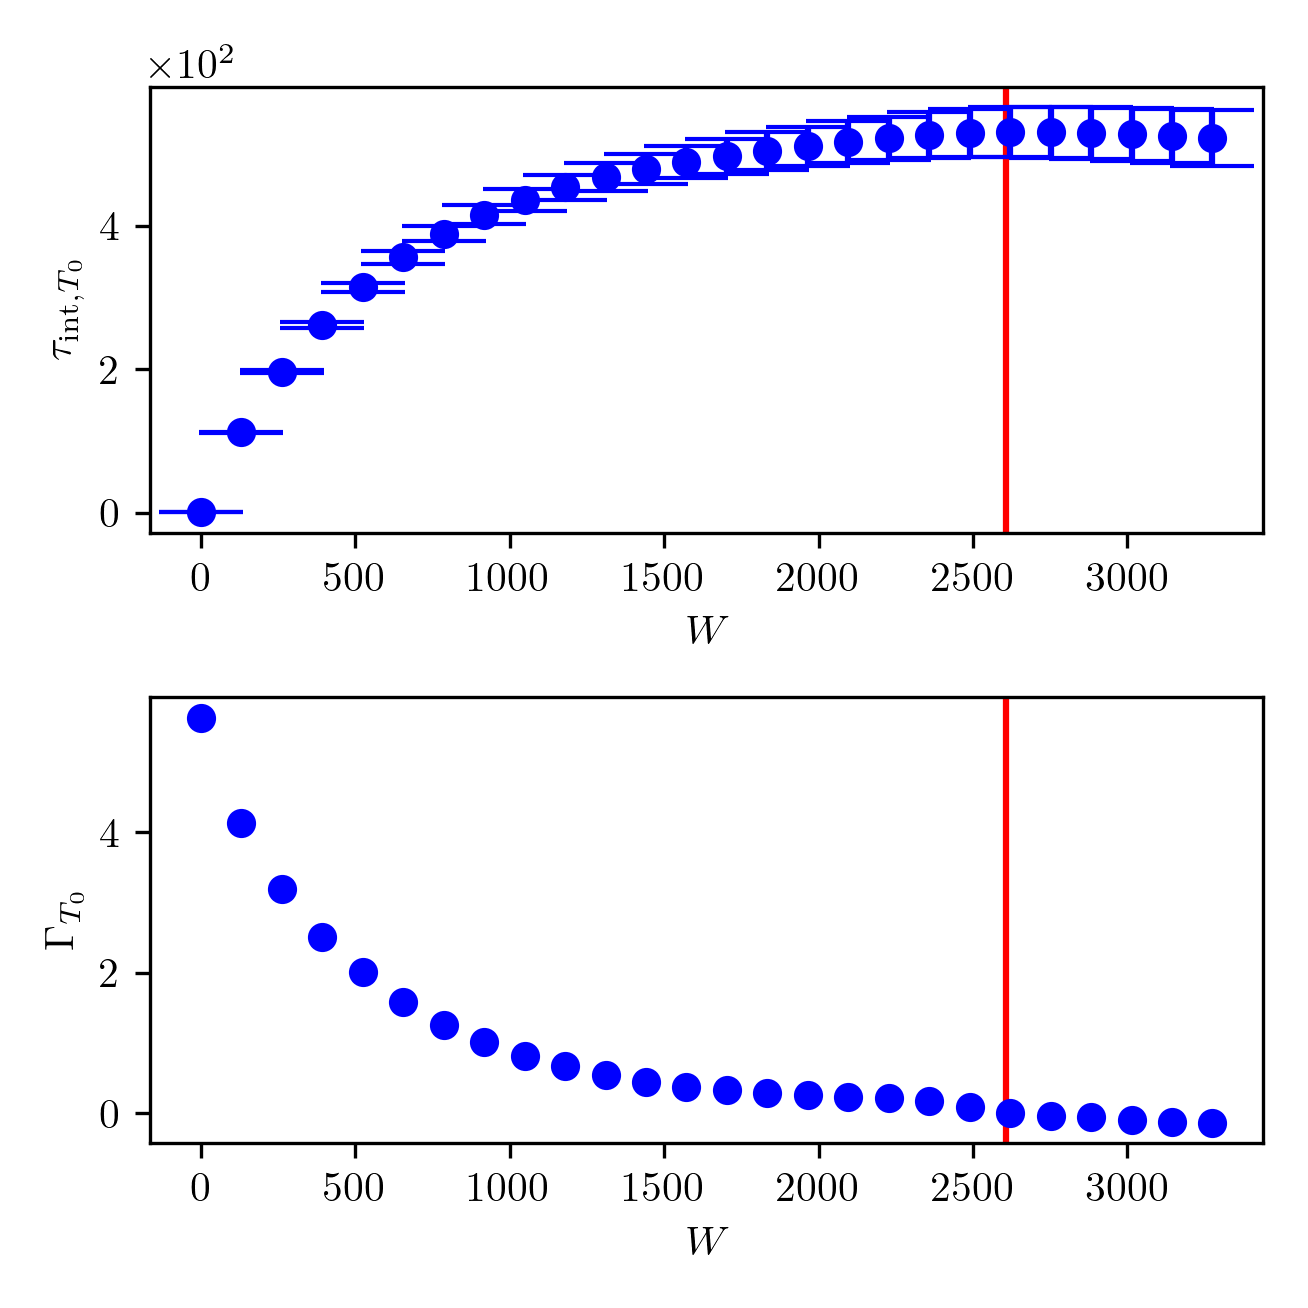
\includegraphics{UwerrTauIntTWalk13.png}
	\caption[IACT and autocorrelation function for $T_0$ samples.]{IACT and autocorrelation function for samples $T_0 \sim \pi( \cdot | h_1, h_2,h_3,h_4,h_5,h_6,a_0,a_1,a_2,a_3,a_4,a_5,a_6,b,p_0,  \bm{y})$}
	\label{fig:}
\end{figure}
\begin{figure}[ht!]
	\centering
	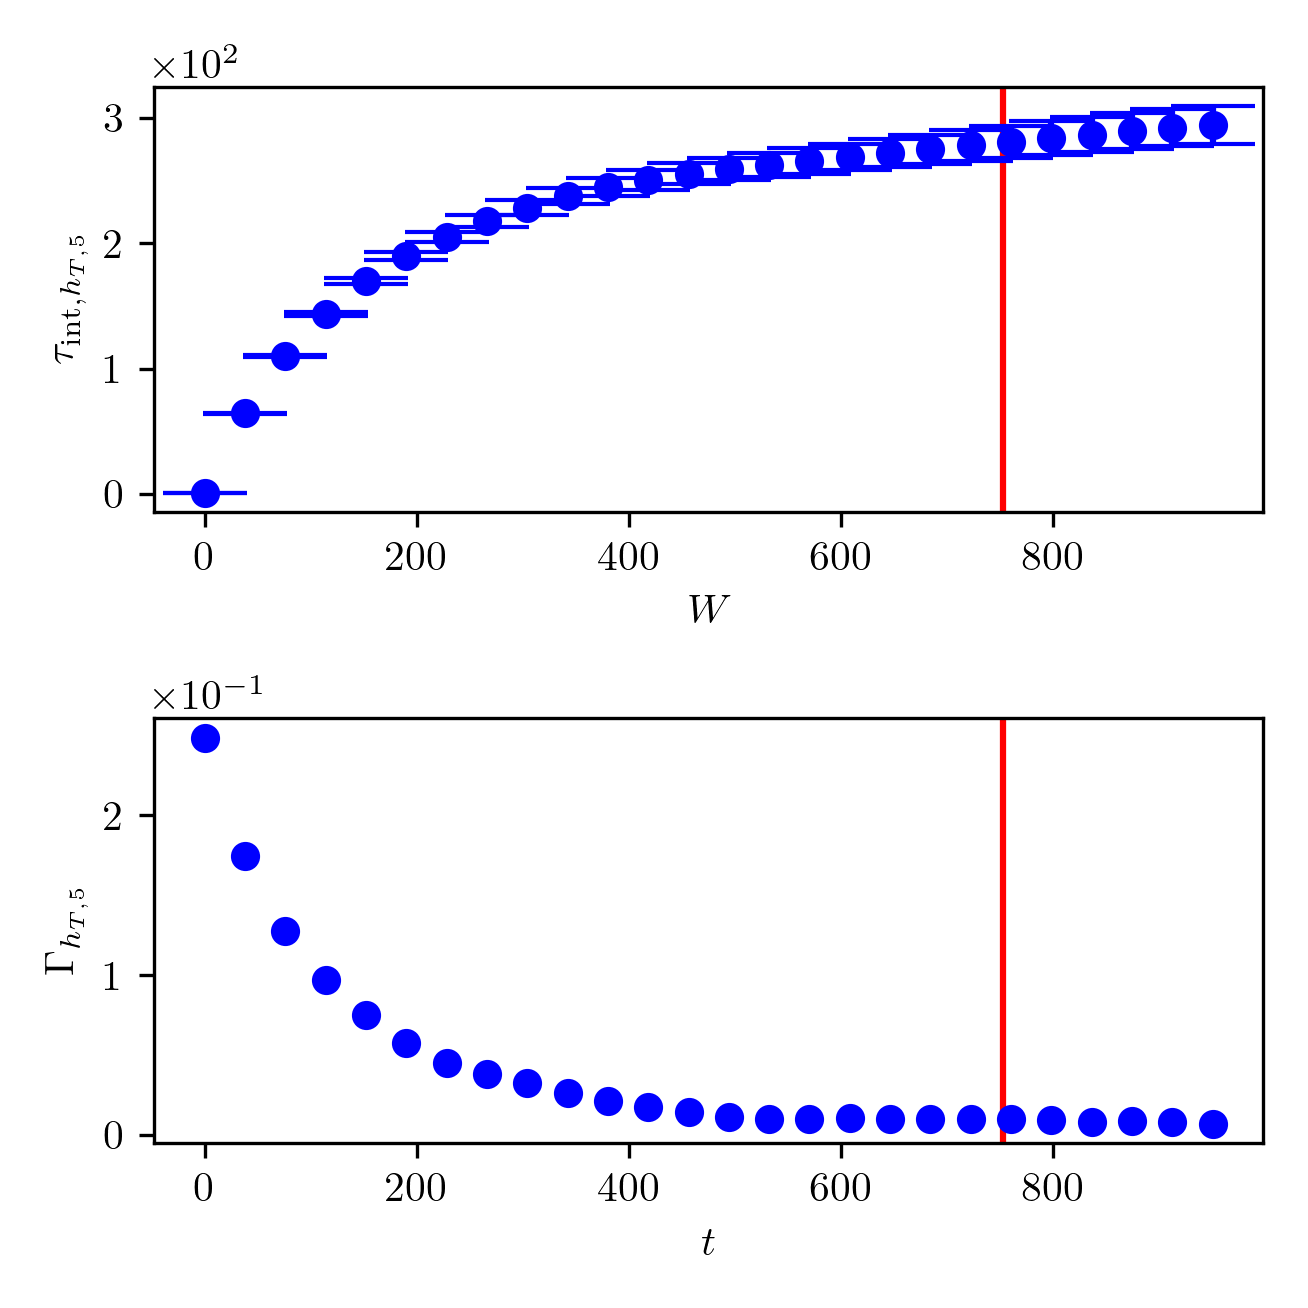
\includegraphics{UwerrTauIntTWalk14.png}
	\caption[IACT and autocorrelation function for $b$ samples.]{IACT and autocorrelation function for samples $b \sim \pi( \cdot | h_1, h_2,h_3,h_4,h_5,h_6,a_0,a_1,a_2,a_3,a_4,a_5,a_6,T_0,p_0,  \bm{y})$}
	\label{fig:}
\end{figure}

\begin{figure}[ht!]
	\centering
	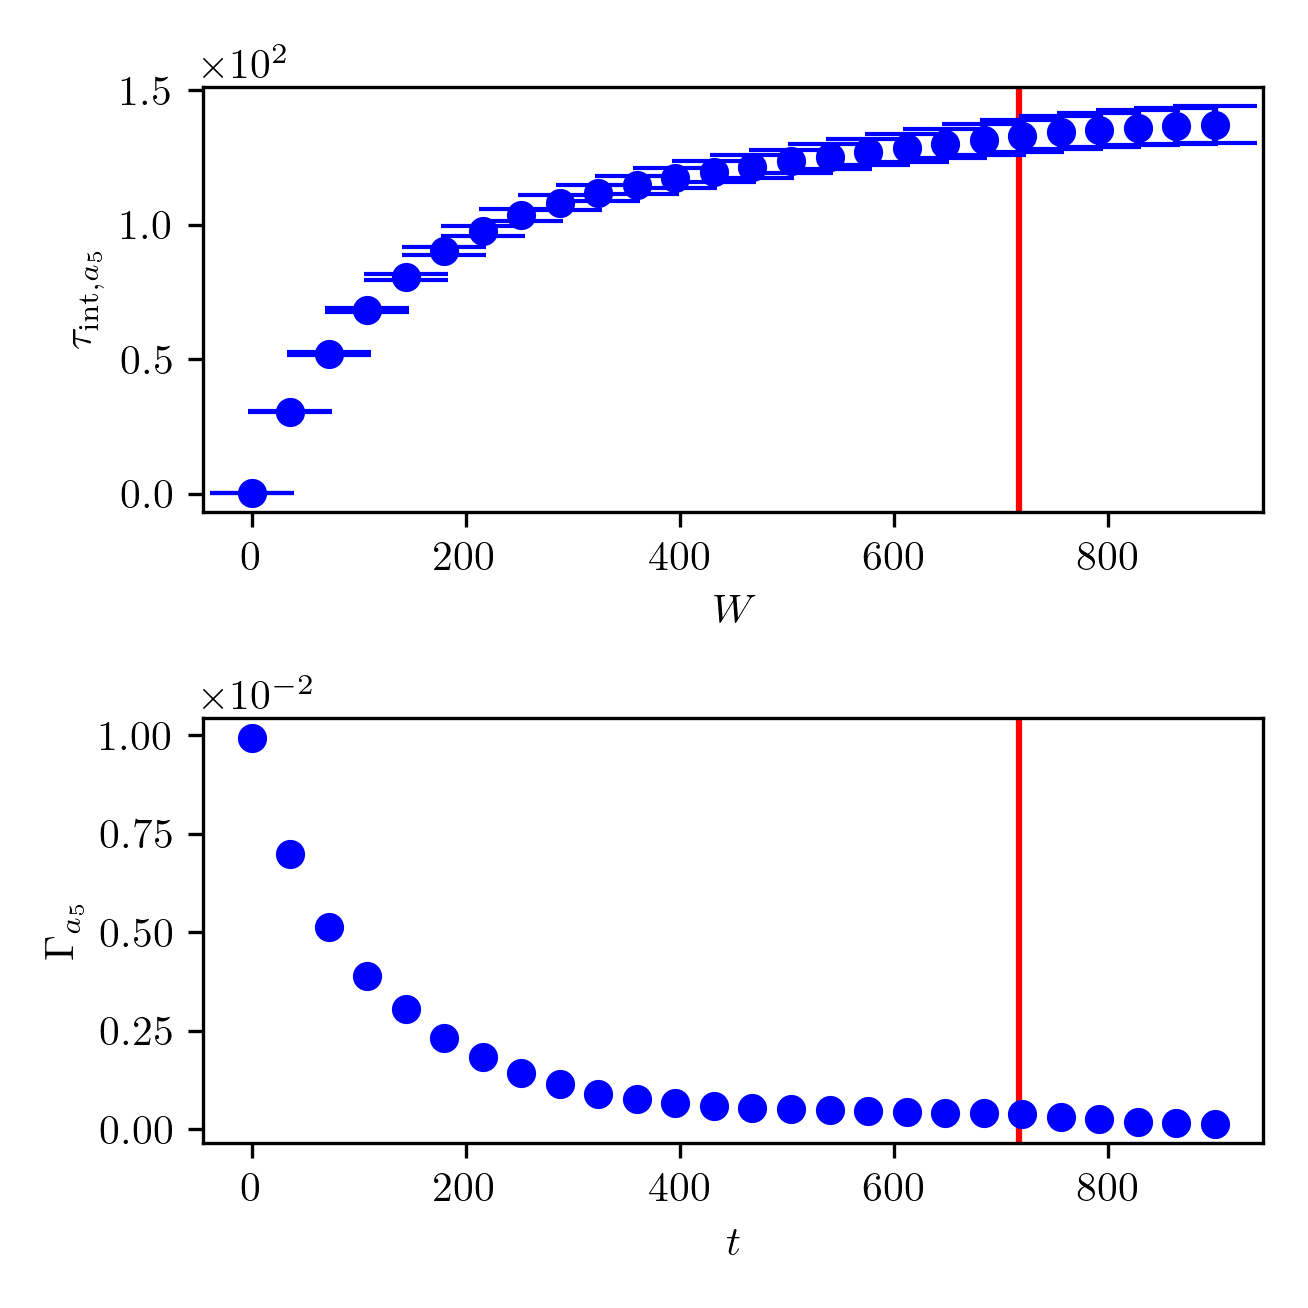
\includegraphics{UwerrTauIntTWalk15.png}
	\caption[IACT and autocorrelation function for $p_0$ samples]{IACT and autocorrelation function for samples $p_0 \sim \pi( \cdot | h_1,h_2,h_4,h_5,h_6,a_0,a_1,a_2,a_3,a_4,a_5,a_6,T_0,b, \bm{y})$}
	\label{fig:}
\end{figure}
\begin{figure}[ht!]
	\centering
	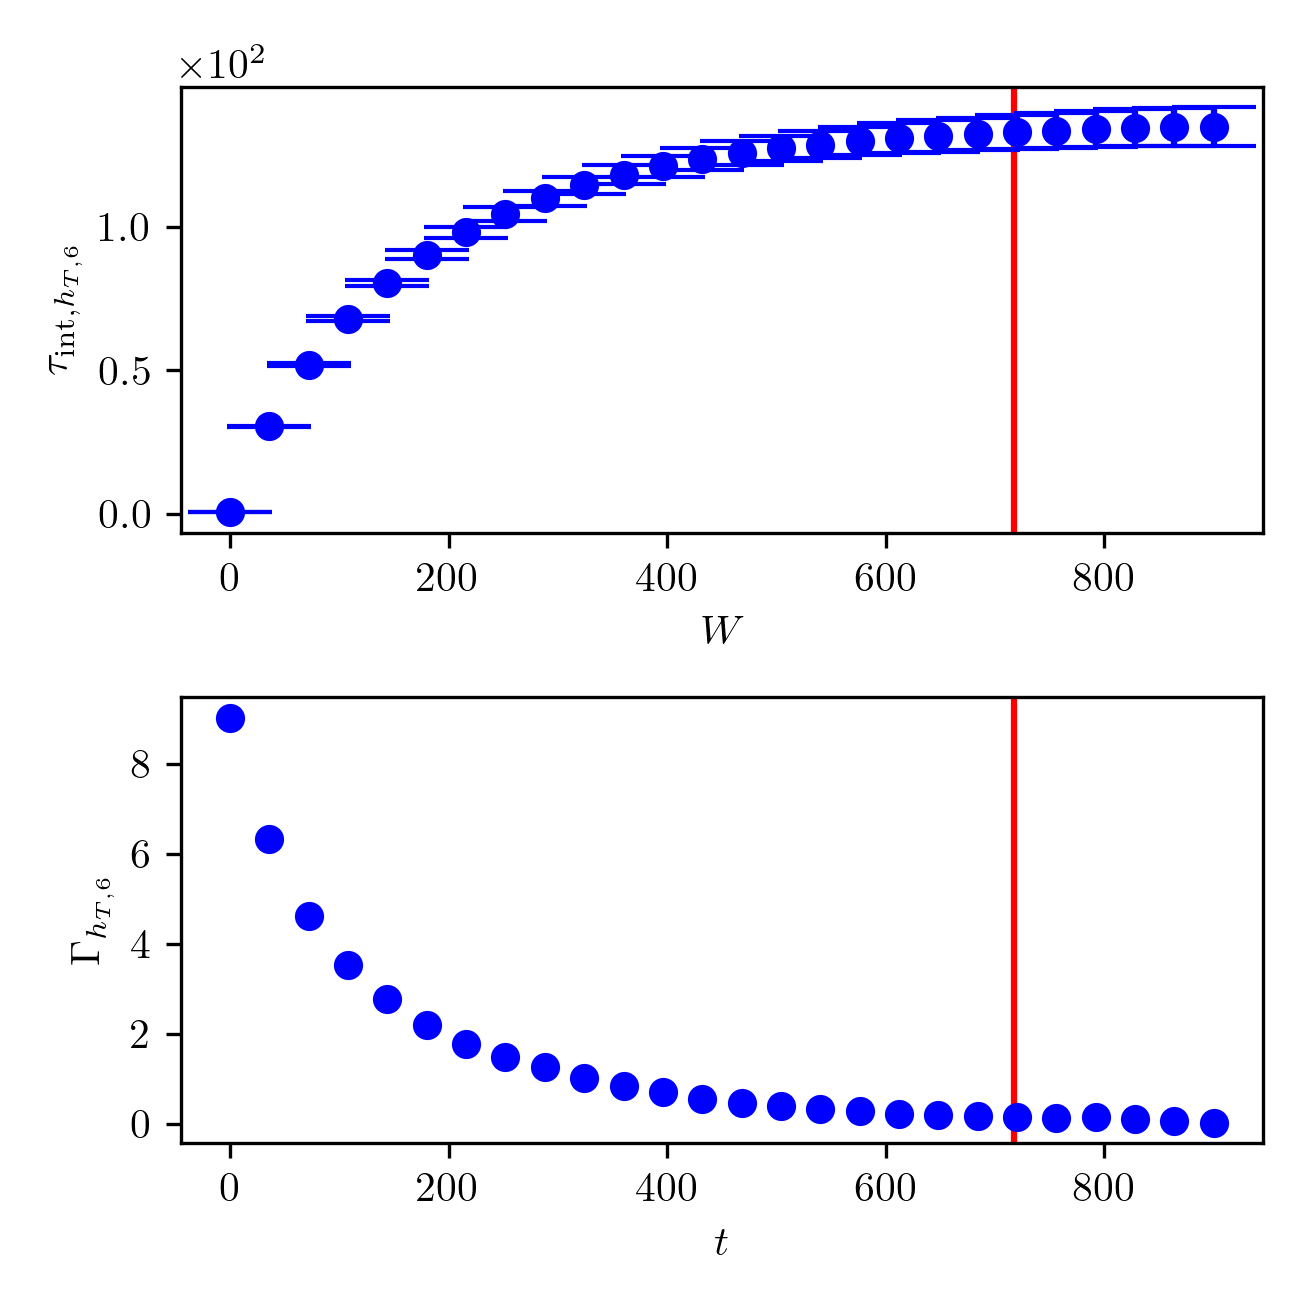
\includegraphics{UwerrTauIntTWalk16.png}
	\caption[IACT and autocorrelation function for $p_0$ samples]{IACT and autocorrelation function for samples $p_0 \sim \pi( \cdot | h_1,h_2,h_4,h_5,h_6,a_0,a_1,a_2,a_3,a_4,a_5,a_6,T_0,b, \bm{y})$}
	\label{fig:}
\end{figure}

\begin{figure}[ht!]
	\centering
	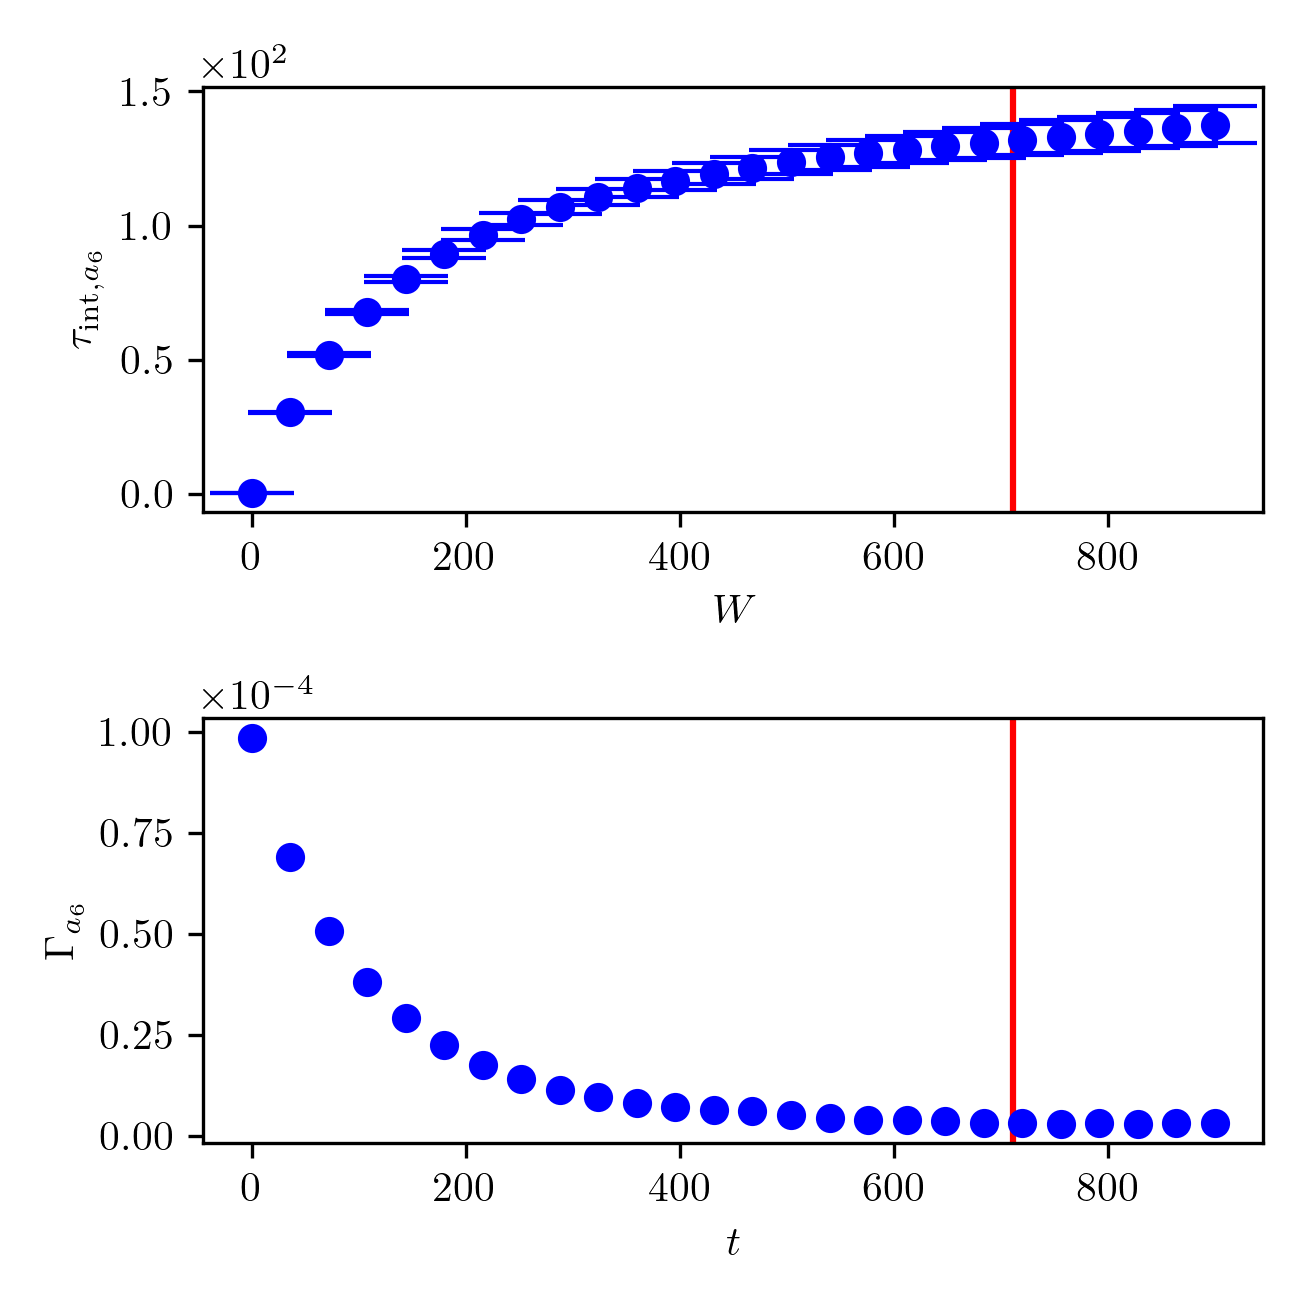
\includegraphics{UwerrTauIntTWalk17.png}
	\caption[IACT and autocorrelation function for $p_0$ samples]{IACT and autocorrelation function for samples $p_0 \sim \pi( \cdot | h_1,h_2,h_4,h_5,h_6,a_0,a_1,a_2,a_3,a_4,a_5,a_6,T_0,b, \bm{y})$}
	\label{fig:}
\end{figure}





